\documentclass[10pt]{article}
\usepackage[T1]{fontenc}
\usepackage{tgadventor}

\usepackage[margin=0.75in]{geometry}
\usepackage{multicol}
\usepackage{titlesec}
\usepackage{xcolor}
\usepackage{svg}
\usepackage{tabularx}
\usepackage{graphicx}
\usepackage{float}
\usepackage{amsmath}
\usepackage{hyperref}
\usepackage{tikz}
\usepackage{fancyhdr}
\usepackage{lastpage}
\usepackage{pgfplots}
\usepackage{subcaption}
\usepackage{dblfnote}
\usepackage[american,siunitx]{circuitikz}
\usepackage[backend=biber, defernumbers=true, sorting=none]{biblatex} %\nocite{*}
\usepackage[font={footnotesize,it},labelfont={footnotesize,it,bf}]{caption}
%\usepackage{indentfirst}
%\usepackage{mathptmx}

% Environmental Settings
\addbibresource{references.bib}
\renewcommand*{\bibfont}{\normalfont\footnotesize}
\graphicspath{{images/}}
\setsvg{inkscapeexe={"C:/Program Files/Inkscape/bin/inkscape.exe"}} % POINT TO /inkscape.exe AS NEEDED
\newcolumntype{C}{>{\centering\arraybackslash}X} % from array package
\usetikzlibrary{positioning, shapes.geometric, patterns, patterns.meta}
\titlespacing*{\section}{0pt}{8pt}{8pt}
\titlespacing*{\subsection}{0pt}{7pt}{7pt}
\titlespacing*{\subsubsection}{0pt}{5pt}{5pt}
\titlespacing*{\paragraph}{0pt}{5pt}{5pt}
\definecolor{copper}{rgb}{0.72, 0.45, 0.2}
\definecolor{forestgreen(traditional)}{rgb}{0.0, 0.27, 0.13}
\definecolor{forestgreen(web)}{rgb}{0.13, 0.55, 0.13}
\definecolor{github-indigo}{RGB}{64, 120, 192}
\definecolor{github-butterfly-bush}{RGB}{110, 84, 148}
\ctikzset{bipoles/buffer/height/.initial=0.8}
\ctikzset{amplifiers/op amp/height/.initial=0.8}
\ctikzset{amplifiers/op amp/length/.initial=0.8}
\tikzset{
    block/.style={
        draw, minimum width = 1cm, 
        minimum height = 0.7cm, 
        align = center,
        font = \footnotesize
    }, 
    every node/.style = {node distance=0.5cm},
    line/.style = {-latex}
}

\begin{document}

    \pagestyle{fancy}
    \fancyhf{}
    \fancyhead[LH]{\footnotesize{Dynamic Range Compressor Design | Goda, Shaun}}
    \fancyhead[RH]{\footnotesize{Technical Report | \today}}
    \renewcommand{\headrulewidth}{0pt}
    \fancyfoot[C]{\footnotesize{Page \thepage\ of \pageref{LastPage}}}
    \fancypagestyle{firstpage}{
        \fancyhf{}
        \fancyfoot[C]{\footnotesize Page \thepage\ of \pageref{LastPage}}
        \renewcommand{\headrulewidth}{0pt}
    }

    \title{
        \vspace{-5ex}
        \textbf{\huge Dynamic Range Compressor Design}\\
        \textit{Technical Report in Analog Signal Processing and Discrete Circuit Design for Applications in Audible Frequency Domain}
    }

    \author{
        \textbf{\Large Shaun Goda}\\
        \textit{\normalsize Department of Electrical and Computer Engineering, Rutgers University - New Brunswick}
    }

    \date{\vspace{-5ex}} % This command effectively gets rid of the date section from \maketitle

    \maketitle

    \thispagestyle{firstpage}

    \begin{abstract}
        This technical report examines the fundamental theory and implementation of dynamic range compressors in the realm of analog signal processing as we embark on a constructional project. Through tests and evaluations, we present methods for achieving efficient and high-performance compressors, where we will start with an overview of the basic building block of the compressor, its representation as a mathematical function, and methods of implementation through analog circuitry. This paper offers an entry point for those looking to understand the fundamentals of how an dynamic range compressor works, while balancing the nuances of the practical methods and challenges associated with developing an electronic hardware device.
    \end{abstract}
    
    \begin{multicols*}{2}

        \textbf{Keywords:} \textit{Signal Processing, Circuit Design,\\Dynamic Range Compression, Analog Circuit, Printed Circuit Board, Signal Integrity.}

        \section{Introduction}
            A dynamic range compressor (DRC) is an essential tool in audio processing that normalizes the loudness of a signal that has been put through. This is done by using a mechanism that attenuates signals above a set threshold, utilizing a variable gain mechanism governed by a level-detection algorithm. The process effectively lowers the volume of louder segments of the audio while maintaining the level of quieter sections, resulting in a more uniform overall loudness. This technology is widely used in various areas such as music production, live performances, and even in devices like hearing aids to improve sound quality.\par
            With the emergence of high-performance computational platforms and advancement in signal processing technologies, digital signal compression algorithms has been a de-facto standard in the industry. Digital compressors are popular in many applications, from creating music to broadcasting and beyond, as they allow for detailed and precise manipulation of sound. The digital transformation of compressors and other signal processing tools has fundamentally changed audio production. Allowing the average consumer to achieve professional-quality production on a personal laptop without the need for an access to a professional recording studio.\par
            Furthermore, despite the dominance of digital signal processing technologies, hardware compressors, where the signal is processed entirely in the analog domain, widely remain in use. Many audio professionals continue to prefer them for certain tasks as it offers various advantage and benefits that has an edge over software implemented compressors.\par
            In comparison to digital compressors, analog compressors are generally valued for the unique qualities they can add to sound. They are known for introducing warmth\footnotemark and musicality to the audio that is often described as being difficult to achieve with digital methods. \cite{sos-warmth} This effect is due to the slight alterations the analog circuits introduce, including minor distortions and saturations, making the audio sound richer and more engaging to the audience. Analog compressors are also favored for its straightforwardness, avoiding some of the issues that digital formats can introduce, such as digital latency caused by AD/DA conversion and process run time. Furthermore, it is advantageous in avoiding issues that are caused by the inherent nature of digital compressors, such as unwanted sampling artifacts, signal aliasing, and the added complexity of software installation and digital library management. Thus, despite the convenience and precision of digital compressors, analog compressors still hold its own place in audio production for their ability to enhance sound in a distinctive way.\par
            In light of the various advantages seen in analog compressors, this paper will delve deeper into the technical nuances and design considerations that underpins an effective analog compressor. By examining the control parameters, exploring the functional building blocks, and discussing various control mechanisms, we aim to investigate the intricate balance between theory and practical application that lies in designing an analog compressor. Furthermore, the following sections highlights the critical decisions and engineering challenges involved in creating an analog compressors that not only meet the technical specifications, but also stands out as an appealing alternative to the widely used digital compressor.

            \vspace{2cm}

            \par\noindent\rule{\linewidth}{0.5pt}
            \begin{minipage}[b]{\linewidth}
                \vspace{2pt}
                \footnotesize{$^1$ The term 'warmth' is often used to refer to the pronounced reverberation time at low frequencies relative to that at higher frequencies.} \cite{britanica-warmth}
            \end{minipage}\hfill

            %\footnotetext{\textit{The term 'warmth' is often used to refer to the pronounced reverberation time at low frequencies relative to that at higher frequencies.\cite{britanica-warmth}}}

        % Compression ratio plot
        \noindent
        \begin{minipage}{\linewidth}
            \centering
            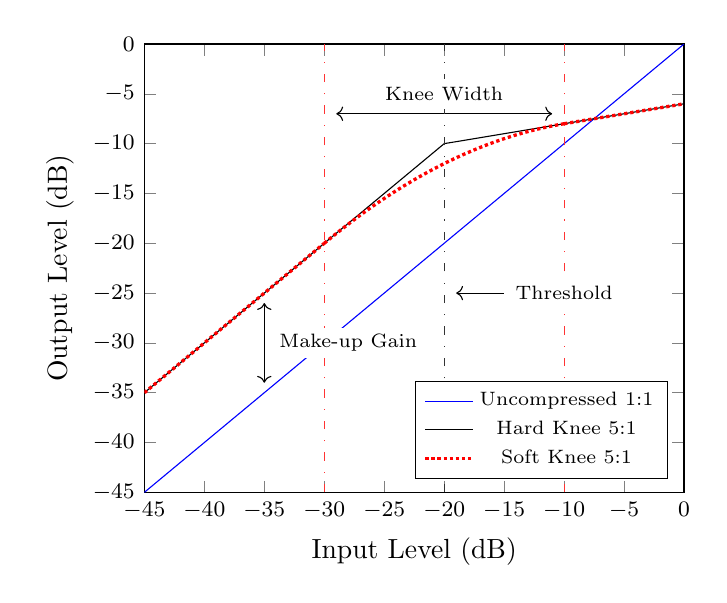
\begin{tikzpicture}
                \begin{axis}[
                    ticklabel style = {font=\footnotesize},
                    xtick distance=5,
                    ytick distance=5,
                    xlabel={Input Level (dB)},
                    ylabel={Output Level (dB)},
                    xmin=-45, xmax=0,
                    ymin=-45, ymax=0,
                    legend pos=south east,
                    %xmajorgrids=true,
                    %ymajorgrids=true,
                    grid style=dashed,
                ]
                
                % No compression line
                \addplot[
                    color=blue,
                    domain=-45:0,
                ] {x};
                
                % 5:1 Compression, hard knee
                \addplot[
                    color=black,
                    solid,
                    domain=-45:-20,
                ] {x + 10};
                \addplot[
                    color=black,
                    solid,
                    domain=-20:0,
                ] {0.2*x-6};
    
                % 5:1 Compression, soft knee
                \addplot[
                    color=red,
                    very thick,
                    densely dotted,
                    domain=-45:-30,
                ] {x + 10};
                \addplot[
                    color=red,
                    very thick,
                    densely dotted,
                    domain=-30:-10,
                ] {-0.02*x^2-0.2*x-8};
                \addplot[
                    color=red,
                    very thick,
                    densely dotted,
                    domain=-10:0,
                ] {0.2*x-6};
                
    
                % Make-up gain
                \draw [<->] (axis cs:-35,-34) -- (axis cs:-35,-26);

                % Knee boundary line
                \draw [color=red!80, loosely dashdotted] (axis cs:-30,-45) -- (axis cs:-30,0);
                \draw [color=red!80, loosely dashdotted] (axis cs:-10,-45) -- (axis cs:-10,0);
                \draw [<->] (axis cs:-29,-7) -- (axis cs:-11,-7);
                
                % Threshold line
                \draw [color=black!80, loosely dashdotted] (axis cs:-20,-45) -- (axis cs:-20,0);
                \draw [->] (axis cs:-15,-25) -- (axis cs:-19,-25);

                \fill [white] (axis cs:-25,-6.5) rectangle (axis cs:-15,-3.5);
                \node at (axis cs:-20,-5){\scriptsize{Knee Width}};

                \fill [white] (axis cs:-15,-27) rectangle (axis cs:-5,-23);
                \node at (axis cs:-10,-25){\scriptsize{Threshold}};

                \fill [white] (axis cs:-34,-31.5) rectangle (axis cs:-22,-28.5);
                \node at (axis cs:-28,-30){\scriptsize{Make-up Gain}};

                \legend{\scriptsize{Uncompressed 1:1},,\scriptsize{Hard Knee 5:1},,\scriptsize{Soft Knee 5:1}};
                
                \end{axis}
            \end{tikzpicture}
            \captionof{figure}{A typical compressor's transfer characteristics, mapped on a decibel scale.}
            \label{fig:comp-ratio}
        \end{minipage}

        \section{Compressor Control Parameters}
            A compressor's functionality is governed by its control parameters, which allow users to configure the effect's characteristics. Key parameters include Threshold, Ratio, Attack, Release, Knee, and Side-chain; each defining a specific aspect of the compressor's behavior and its impact on the input signal.

            \paragraph{Threshold}
                The threshold parameter sets the level at which the compressor starts to act. Measured in decibels (dB), it defines the point above which the input signal will be compressed. When the signal level exceeds this threshold, compression is applied.

            \paragraph{Ratio}
                The ratio determines the degree of compression applied to an audio signal once it exceeds a predetermined threshold level. This parameter is quantified as a ratio, such as 5:1 or 10:1, extending to infinity:1, at which point the compressor operates as a limiter, equalizing all signal levels above the threshold to a consistent amplitude. For instance, a 5:1 ratio signifies that for every increment of 5 dB by which the input signal surpasses the threshold, the output signal's level will be attenuated by only 1 dB. Consequently, higher ratios yield more pronounced compression.

                \begin{equation} \label{eq:ratio}
                    R=\frac{y_{dB}-T}{x_{dB}-T}
                \end{equation}

                \noindent Equation \ref{eq:ratio} mathematically models the compression ratio $R$, where $x_{dB}$ represents the input level gain, $y_{dB}$ the output level gain, and $T$ being the threshold. This formula dictates the change in output level for a given change in input level, relative to the threshold, providing a precise numerical value for the compression effect. The closer the value of $R$ is to 1, the more subtle the compression, while larger values indicate more aggressive compression, leading to the limiting effect.

                % Transient response diagram
                \noindent
                \begin{minipage}{\linewidth}
                    \centering
                    \includesvg[inkscapelatex=false,width=0.935\linewidth]{attack-release-trans.svg}
                    \captionof{figure}{Transient response of a signal through a compressor.}
                    \label{fig:comp-trans}
                \end{minipage}\\

            \paragraph{Attack}
                The attack time determines the time it takes for the compressor to start acting after the signal exceeds the threshold, as seen in the 'attack phase' section of figure \ref{fig:comp-trans}. It is usually measured in milliseconds (ms). A fast attack time means the compressor responds quickly to level changes, suitable for controlling sharp, transient sounds. A slower attack allows some of the initial transients through, preserving more of the signal's natural character.

            \paragraph{Release}
                Release time refers to the duration needed for the compressor to cease its action once the signal dips below the threshold. (as illustrated in Figure \ref{fig:comp-ratio}) This period, also expressed in milliseconds, influences the sound's dynamics; a brief release time halts the compression swiftly, preserving the natural dynamics but may lead to noticeable fluctuations in volume. Conversely, an extended release time ensures a more seamless and gradual transition back to the uncompressed sound.

            \paragraph{Knee}
                The knee parameter (measured in dB in reference to the difference in the lower and upper bound of the knee) precisely controls the compressor's transition from the uncompressed to the compressed state by adjusting its width, which measures how the compression ratio is applied at around the threshold level. A 'hard knee' setting indicates an immediate application of the compression ratio as soon as the signal crosses the threshold, resulting in an abrupt transition. Conversely, a 'soft knee' setting allows for a gradual introduction of compression as the signal nears and surpasses the threshold, due to a wider knee width. The control over the knee width allows the user to achieve a smoother, more natural compression effect, making the transition less noticeable and more musically pleasing.
            
            \paragraph{Make-Up Gain}
                Make-up gain is a control parameter that allows you to increase the output level of the signal after it has gone through compression. This feature helps the user with adjusting the output to a consistent volume level after the signal has undergone attenuation by the compression algorithm. In the context of a song or an audio program, it allows the user to enhances the presence of the material.

            \paragraph{Side-chain}
                Side-chain is a control that is established by passing an additional audio signals to trigger the compression on the main input signal. This technique allows the compressor to react not to its own input signal, but to the dynamics of another, offering creative applications such as ducking, where the volume of one sound is reduced by the presence of another (e.g., background music lowering when someone speaks). It's a powerful tool for achieving more complex mixing and mastering effects, enhancing clarity, and creating rhythmic variations in audio production.

        \section{Compressor Topology} \label{sec:comp-tpgy}
            The method of attenuation seen in a compressor could be generally categorized into two topologies including feedback and feed-forward compression. Both topologies can be expressed as a relation described in equation \ref{eq:gen-topology}, where the output, $y_{dB}$, is given by the sum of input, $x_{dB}$, and the gain/attenuation level, $g_{dB}$, which is determined by the gain computer. 

                \begin{equation} \label{eq:gen-topology}
                    y_{dB}(t)=x_{dB}(t)+g_{dB}(t)
                \end{equation}
            
            \noindent The topology of an compressor fundamentally influences the performance, sound characteristics, and functionality of dynamic range compressors. Such influences can be seen in factors such as how quickly a compressor reacts to signal changes, the smoothness or aggressiveness of compression.

            \subsection{Feedback Compression}
                In a feedback topology, the output signal is looped back and used as part of the signal processing chain as shown in figure \ref{fig:feedback}. Assuming a hard knee with no attack or release, equation \ref{eq:feedback} models the output of the gain computer in such topology.\par

                    \begin{equation} \label{eq:feedback}
                        g_{dB}=(1-R)(y_{dB}-T)
                    \end{equation}
                
                \noindent In general, the feedback topology allows for the compressor to react to the processed signal, enabling a more adaptive response to the audio material. Furthermore, the inherent nature of the feedback system ensures that the compressor's adjustments are directly influenced by its own output, leading to a smoother and more consistent control over dynamic range.\par
                However, the design of the feedback mechanism also presents several limitations, including the lack of a look-ahead capability and its ineffectiveness as an ideal limiter, as it would require an infinite negative amplification applied at the gain computer stage.

                    % Feedback diagram
                    \noindent
                    \begin{minipage}{\linewidth}

                        \centering

                        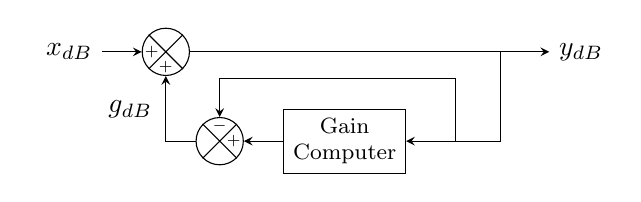
\begin{tikzpicture}

                            \node (input) at (0,0) {$x_{dB}$};
                            \node (output) at (6.5,0) {$y_{dB}$};

                            % Sum1 shape
                            \node[draw,
                                circle,
                                minimum size=0.6cm,
                                right = of input,
                            ] (sum1) {};
                            \draw (sum1.north east) -- (sum1.south west) (sum1.north west) -- (sum1.south east);
                            \node[left=-1pt] at (sum1.center){\tiny $+$};
                            \node[below] at (sum1.center){\tiny $+$};       
                            
                            % Sum2 shape
                            \node[draw,
                                circle,
                                minimum size=0.6cm,
                                below right = 0.7 and 0.25 of sum1,
                            ] (sum2) {};
                            \draw (sum2.north east) -- (sum2.south west) (sum2.north west) -- (sum2.south east);
                            \node[above] at (sum2.center){\tiny $-$};
                            \node[right=-1pt] at (sum2.center){\tiny $+$};
                
                            % Gain Computer
                            \node[block, right = of sum2] (gain) {Gain\\Computer};

                            % Lines
                            \draw[-stealth] (input) -- (sum1.west);
                            \draw[-stealth] (sum1.east) -- (output) node[left = of output](split1){};
                            \draw[-stealth] (sum2.west) -| (sum1.south);
                            \draw[-stealth] (gain.west) -- (sum2.east);
                            \draw[-stealth] (split1.center) |- (gain.east) node[right = of gain](split2){};
                            \draw[-stealth] (split2) -| +(0,0.8) -| (sum2.north);
                            
                            \node[below left = 0.5 and 0.05 of sum1.center] (g_db) {$g_{dB}$};

                        \end{tikzpicture}
                            
                        \captionof{figure}{Control diagram of a feedback compressor topology.}
                        \label{fig:feedback}
                    
                    \end{minipage}
                
            \subsection{Feed-forward Compression}
                As opposed to the feedback topology, feed-forward topology uses the input signal directly to control the compression process, without the influence of the compressed signal in the control loop. (As seen in figure \ref{fig:feedforward}) This allows for more precise and immediate control over the compression characteristics, as the system's response is solely based on the incoming audio signal.\par

                    \begin{equation}\label{eq:feedforward}
                        g_{dB}=(\frac{1}{R}-1)(x_{dB}-T)
                    \end{equation}
                    
                \noindent The gain computer's output, $g_{dB}$ can be modeled by the equation \ref{eq:feedforward}, and when in comparison to equation \ref{eq:feedback}, it can be shown that the inherent issue seen in requiring an infinite amplification is no longer a problem in feed-forward topology as the slope for the limiter simply reaches a slope of -1. For this reason, many modern implementation of the both digital and analog compressor rely on the feed-forward variant.

                    % Feed-forward diagram
                    \noindent
                    \begin{minipage}{\linewidth}

                        \centering

                        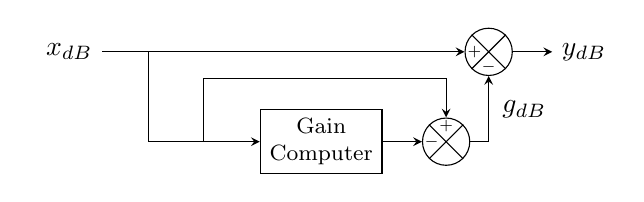
\begin{tikzpicture}

                            \node (input) at (0,0) {$x_{dB}$};

                            % Gain Computer
                            \node[block, below right = 0.5 and 2 of input] (gain) {Gain\\Computer};

                            % Sum1 shape
                            \node[draw,
                                circle,
                                minimum size =0.6cm,
                                right = of gain,
                            ] (sum1) {};
                            \draw (sum1.north east) -- (sum1.south west) (sum1.north west) -- (sum1.south east);
                            \node[left=-1pt] at (sum1.center){\tiny $-$};
                            \node[above] at (sum1.center){\tiny $+$};       
                            
                            % Sum2 shape
                            \node[draw,
                                circle,
                                minimum size = 0.6cm,
                                right = 4.6cm of input,
                            ] (sum2) {};
                            \draw (sum2.north east) -- (sum2.south west) (sum2.north west) -- (sum2.south east);
                            \node[left=-1pt] at (sum2.center){\tiny $+$};
                            \node[below] at (sum2.center){\tiny $-$};
                
                            % Lines
                            \draw[-stealth] (input) -- (sum2.west);
                            \draw[-stealth] (1,0) |- (gain.west) node[near end](split){};
                            \draw[-stealth] (gain.east) -- (sum1.west);
                            \draw[-stealth] (split) -| +(0,0.8) -| (sum1.north);
                            \draw[-stealth] (sum1.east) -| (sum2.south);
                            \draw[-stealth] (sum2.east) -- +(0.5,0) node[right]{$y_{dB}$};

                            \node[below right = 0.5 and 0.05 of sum2.center] (g_db) {$g_{dB}$};
                            
                        \end{tikzpicture}
                        
                        \captionof{figure}{Control diagram of a feed-forward compressor topology.}
                        \label{fig:feedforward}
                    
                    \end{minipage}

            \subsection{Additional Topologies}
                In addition to feed-forward and feedback topologies, there are other variations in where an compressor can be implemented. Such topology often includes\dots

                \subsubsection{Upward compression}
        
                \subsubsection{Broadband, Multiband, and Spectral Compression}
                    Broadband compressors operate by adjusting the dynamics of an input signal across the entire frequency range; when a set threshold is exceeded, the entire signal is affected, regardless of the specific frequencies composing the signal's energy.\par
                    Differing from this approach, a multiband compressor divides the entire frequency spectrum into multiple bands that can be independently adjusted. This allows for more flexible and significant compression of a single track or instrumental group without the risk of making extensive changes too audibly noticeable. \par
                    On another front, spectral compressors continuously analyze the spectral distribution of a signal's energy and compare it with target values determined by intelligent algorithms. When the system identifies that certain frequency areas are being overemphasized, thus disproportionately affecting the compression, those areas are automatically subjected to more intense compression.

        \section[Functional Building Blocks of a Compressor]{Functional Building Blocks\\of a Compressor}
            The inner components that consist the functionality of a compressor can be mainly separated into three sections, including the output amplifier, compression calculator, and the level detector. Where the output amplifier takes the role of directly adjusting the amplitude of the compressor, the compression calculator and the level detector (consisting the gain computer) is responsible of generating the control signal for the output amplifier that varies the attenuation level. Within this section, various implementation of output amplifier, compression calculator, and the level detector is examined.

            \subsection{Compression Calculator}
                The gain computer is responsible for generating the control voltage, which dictates the gain reduction level applied to the signal. This stage is based on determining amplitude-based parameters of the attenuation generated by the gain computer, including Threshold (T), Ratio (R), and Knee Width (W), where its relation in regards to the output of the gain computer is described by a set of bounded equations shown in equation \ref{eq:gain-comp}.

                    % Expression of knee control in terms of 
                    \begin{equation}
                        y=
                        \begin{cases}
                            \frac{x-T}{R}+T & \text{for $2(x-T)>W$}\\[5pt]
                            \frac{(x-T+\frac{W}{2})^2(\frac{1}{R}-1)}{2W}+x & \text{for $2\left\lvert x-T\right\rvert\leq W$}\\[5pt]
                            x & \text{for $2(x-T)<-W$}
                        \end{cases}
                        \label{eq:gain-comp}
                    \end{equation}

                When the knee width is set to zero, the smooth knee is identical to the hard knee.
            
            \subsection{Level Detector} \label{sect:lvl-det}
                The level detector is responsible for providing a representation of the loudness of the input signal, where its output function is mainly based on operating time-varying (often introducing delay) functions on the input. Two main implementations of the level detectors are commonly seen in compressors including the peak detector and the RMS detector. Such detectors are employed to ensure a consistent depiction of the signal's intensity and can be implemented at multiple points within the side-chain based on the topology later discussed in \ref{reference to section}.
                
                \subsubsection{Peak Reading Detector}
                    The peak reading detector is crucial for capturing the maximum amplitude of the input signal within a specified time-frame, ensuring the dynamic range of audio material is maintained without clipping. Furthermore, a variant on the standard peak detector, called a quasi-peak detector, are often used in the context of compressors, where attack and release time can be incorporated by incorporating a charge-storing component. (as shown in figure \ref{fig:lossy-peak-det})

                        % Lossy peak detector diagram
                        \noindent
                        \begin{minipage}{\linewidth}
                            \centering
                            \begin{circuitikz}[scale = 0.8, transform shape]
                                \draw
                                (0,0) node[left]{Input}
                                (0,0) to[empty diode, *-] (2,0)
                                to[R, l_=$R_A$] (4,0)
                                to[short] (5,0)
                                to[C, l_=$C$] (5,-2) node[sground]{}
                                (5,0) to[short] (6.5,0)
                                to[R, l_=$R_R$] (6.5,-2) node[sground]{}
                                (6.5,0) to[short, -*] (7.5,0)
                                (7.5,0) node[right]{Output}
                                ;
                            \end{circuitikz}
                            \captionof{figure}{Circuit diagram of a lossy peak detector.}
                            \label{fig:lossy-peak-det}
                        \end{minipage}

                    \noindent In the configuration shown, the diode allows current to flow in one direction, charging the capacitor to the peak voltage level of the input signal. The resistor provides a discharge path for the capacitor, setting the time it takes for the detector to respond to changes in signal level. This arrangement captures and holds the maximum amplitude of the signal momentarily, allowing the compressor circuitry to adjust the gain based on this peak value.\par

                    While highly effective at preserving signal transients, its primary disadvantage lies in its potential to cause overly conservative gain reduction in compressors, as it responds to transient peaks that may not reflect the overall perceived loudness. This can sometimes result in less natural compression effects, as it disregards the human ear's time-based perception of loudness.  
                    
                \subsubsection{Average Reading Detector}
                    The average reading detector is designed to capture the mean amplitude of an input signal over a defined time period, providing a measure that reflects the general level of the signal rather than its peak values. This approach is particularly useful in applications where the overall energy of the signal, rather than its instantaneous peaks is of interest.\par
                    The operation of an average reading detector can be implemented by simply removing the rectification stage (diode) where the signal is directly passed through a low-pass filter to obtain a DC level proportional to the average amplitude of the input waveform. 
                
                \subsubsection{RMS Reading Detector}
                    Utilizing the root mean square (RMS) value of the input signal is particularly helpful when you would like to reference the average power of the input signal, which is more aligned with how our ears perceive loudness. Unlike peak detection, the output of the RMS reading detector has an affect on the both transient and amplitude of the output, where its continuous form expression is defined by equation \cite{aes-that-rms}.
                    
                        \begin{equation}
                            V_{RMS} = \lim_{T \to \infty}\sqrt{\frac{1}{T}\int_{-\infty}^{T} v_{in}^2(t) \,\cdot dt}
                        \end{equation}
                    
                    \noindent RMS detection ensures more consistent levels throughout the audio material, as it's less influenced by short transient peaks, and is suited for providing a more musical and natural-sounding compression. Additionally, the RMS detector offers an edge over the average reading detector particularly in their ability to provide true measurements of power across a variety of waveform types as highlighted in table \ref{table:ave-err}.

                        % RMS and peak comparison table
                        \begin{table*}[!th]
                            \centering
                            \begin{tabularx}{\textwidth}{|l*{4}{|C}|}
                                \hline
                                Type of Waveform (1V Peak Amplitude) & Crest Factor $(V_{Peak}/V_{RMS})$ & RMS value & Average Reading Circuit & Error (\%) \\ \hline
                                Undistorted Sine Wave & 1.414 & 0.707 & 0.707 & 0 \\    \hline
                                Gaussian Noise & 3 & 0.333 & 0.295 & -11.4 \\   \hline
                                Undistorted Triangle Wave & 1.73 & 0.577 & 0.555 & -3.8 \\   \hline
                                Gaussian Noise (98\% of Peaks<1V) & 3 & 0.333 & 0.295 & -11.4 \\    \hline
                                Rectangular & 2 & 0.5 & 0.278 & -44 \\    \hline
                                Pulse Train & 10 & 0.1 & 0.011 & -89 \\    \hline
                                SCR Waveform (50\% Duty) & 2 & 0.354 & 0.354 & -28 \\    \hline
                                SCR Waveform (25\% Duty) & 4.7 & 0.212 & 0.150 & -30 \\    \hline
                            \end{tabularx}
                            \caption{Error introduced by an average responding circuit when measuring common waveforms.}
                            \label{table:ave-err}
                        \end{table*}    

                    Furthermore, utilizing the RMS value may falls short compared to peak reading detectors as it may not react quickly enough to fast input transient, which can lead to unwanted distortion or clipping if the peaks are not adequately managed. Additionally, due to the function of RMS value being based on an indeterminate time ranging from the $t=0$ to $\infty$, it comes at a cost of abandoning control parameters such as attack and release in the context of implementing compressors.

            \subsection{Output Amplifier}
                The gain control in a dynamic range compressor can be achieved by using a voltage controlled amplifier (VCA) where its gain factor is modulated by a control voltage generated by the level detection circuitry. The VCA adjusts the signal's gain based on this control voltage, which reflects the signal's amplitude relative to the compressor's parameters (threshold, ratio, attack, release).
        
        \section[Optimizing Compressor Performance]{Optimizing Compressor\\Performance}
            
            \subsection{Compressor Topology Selection}
                Both feedback and feed-forward topologies offer unique benefits and are chosen based on the specific requirements of the application. However, due to the inherent setback seen in feed-forward topology where it requires an infinite level of amplification to achieve perfect limiting, (as discussed in section \ref{sec:comp-tpgy}) the feedback variant remains a more precise and popular option in the modern day.\par
                Furthermore, the feed-forward topology can be further sub-categorized based on the placement of the level detector and the transient shaping component, as shown in figure \ref{figure to be inserted}.

                    \begin{eqnarray}
                        x_G(t)&=&20log_{10}|x(t)|\\
                        x_L(t)&=&x_G(t)-y_G(t)\\
                        x_{dB}(t)&=&-y_L(t)
                    \end{eqnarray}

                    % Control diagram of compressor to be implemented
                    \begin{figure*}[!th]

                        \centering
                        
                        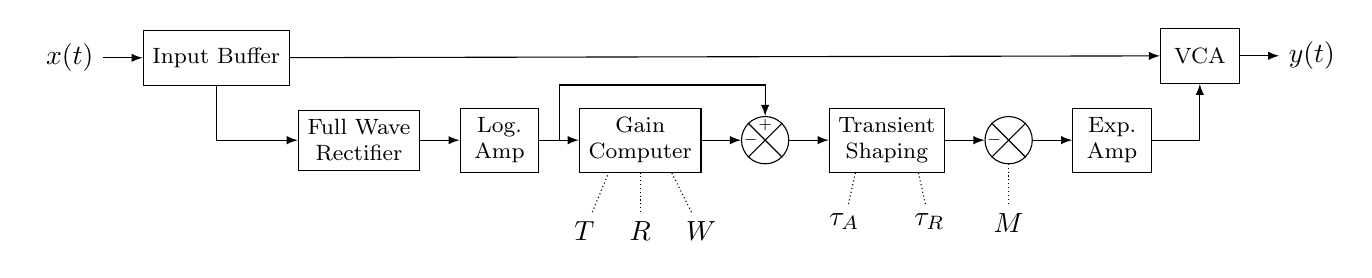
\begin{tikzpicture}
                                
                            \node (input) at (0,0) {$x(t)$};
                                                    
                            % Blocks
                            \node[block, right = of input] (inBuf) {Input Buffer};
                            \node[block, below right = 0.3 and 0.1 of inBuf] (abs) {Full Wave \\ Rectifier};
                            \node[block, right = of abs] (log) {Log. \\ Amp};
                            \node[block, right = of log] (th) {Gain\\Computer};

                            % Sum1 shape
                            \node[draw,
                                circle,
                                minimum size=0.6cm,
                                right = of th,
                            ] (sum1) {};
                            \draw (sum1.north east) -- (sum1.south west) (sum1.north west) -- (sum1.south east);
                            \node[left=-1pt] at (sum1.center){\tiny $-$};
                            \node[above] at (sum1.center){\tiny $+$}; 

                            %\node[block, below = of peak] (rms) {RMS Detector};
                            \node[block, right = of sum1] (peak) {Transient\\Shaping};
                            
                            % Sum2 shape
                            \node[draw,
                                circle,
                                minimum size=0.6cm,
                                right = of peak,
                            ] (sum2) {};
                            \draw (sum2.north east) -- (sum2.south west) (sum2.north west) -- (sum2.south east);
                            \node[left=-1pt] at (sum2.center){\tiny $-$};

                            % Additional blocks
                            \node[block, right = of sum2] (antilog) {Exp. \\ Amp};
                            \node[block, above right = 0.3 and 0.1 of antilog] (vca) {VCA};
                            \node[right = of vca] (output) {$y(t)$};

                            % Lines
                            \draw[line] (input.east) -- (inBuf);
                            \draw[line] (inBuf) |- (abs);
                            \draw[line] (abs) -- (log);
                            \draw[line] (log) -- (th) node[midway](split) {};
                            \draw[line] (th) -- (sum1.west);
                            \draw[line] (split) -| +(0,0.7) -| (sum1.north);
                            \draw[line] (sum1.east) -- (peak);
                            \draw[line] (peak) -- (sum2.west);
                            \draw[line] (sum2.east) -- (antilog);
                            \draw[line] (antilog) -| (vca);
                            \draw[line] (inBuf) -- (vca);
                            \draw[line] (vca) -- (output);        

                            % Arrows and labels for T, R, W
                            \node[below = 0.5cm of th] (r) {$R$};
                            \node[left = 0.2cm of r] (t) {$T$};
                            \node[right = 0.2cm of r] (w) {$W$};
                            \draw[densely dotted] (t) -- ([xshift=-0.4cm]th.south);
                            \draw[densely dotted] (r) -- (th.south);
                            \draw[densely dotted] (w) -- ([xshift=0.4cm]th.south);

                            % Arrows and labels for tau_A, tau_R
                            \node[below = 0.5cm of peak] (cent) {};
                            \node[left = 0.1cm of cent] (tauA) {$\tau_A$};
                            \node[right = 0.1cm of cent] (tauR) {$\tau_R$};
                            \draw[densely dotted] (tauA) -- ([xshift=-0.4cm]peak.south);
                            \draw[densely dotted] (tauR) -- ([xshift=0.4cm]peak.south);
                            
                            % Arrows and labels for M
                            \node[below = 0.5cm of sum2] (m) {$M$};
                            \draw[densely dotted] (m) -- (sum2.south);
                            
                        \end{tikzpicture}

                        \caption{System diagram of a proposed analog DRC system.}
                        \label{fig:drc-diagram}

                    \end{figure*}
    
            \subsection{Logarithmic Domain Signal Processing}
                The perception of loudness by the human ear exhibits a relation that can be mapped to the logarithmic scale. This characteristic implies that as sound levels increase, our sensitivity to changes in volume diminishes. Leveraging this understanding, by converting the input signal into a logarithmic scale before it is processed by the gain computer, we enable the compressor to modulate functions such as knee width compression in alignment with the perceived loudness rather than the signal's linear amplitude. This approach ensures that compression adjustments correlate more closely with human auditory perception.\par
                Furthermore, in the realm of transient shaping, circuits like the peak detection circuit utilize the natural delay inherent in the charging and discharging cycles of a capacitor. The behavior of this cycle, especially its amplitude within a RC network, is mathematically described by equation \ref{eq:lin-cap-discharge}.
                
                    \begin{equation}\label{eq:lin-cap-discharge}
                        V(t) = V_0 e^{-\frac{t}{RC}}
                    \end{equation}    
                
                \noindent This equation delineates how the voltage across a capacitor decays exponentially over time. However, this exponential decay can result in a perceptually unnatural volume decrease, an artifact that could potentially detract from the desired sound quality. By transitioning the signal processing to a logarithmic domain, we can mitigate this issue. Transforming the original equation into a logarithmic form yields equation \ref{eq:log-cap-discharge}.
                
                    \begin{equation}\label{eq:log-cap-discharge}
                        \ln(V(t)) = \ln(V_0) - \frac{t}{RC}
                    \end{equation}
                
                \noindent In this logarithmic representation, the exponential decay of voltage—and consequently, of perceived volume—is linearized. This adjustment facilitates a more natural and smoother compression effect when deploying peak-detection based circuits, aligning the signal processing more closely with the nuances of human auditory perception. 
                
            \subsection{Side-Chain Filtering}
                Side-chain filtering can be introduced to limit the range of frequency the gain computer perceives. This functionality is particularly useful in emphasizing or de-emphasizing, which tells the compressor to be more sensitive or less sensitive to a specific range of frequencies.
                As an example, a high-pass filter might be applied to prevent low-frequency content from triggering the compression, which is particularly useful for avoiding unnecessary compression due to bass-heavy elements in a mix. \cite{side-chain-filtering}\par
                Pre-detection filtering allows for more targeted and musically relevant compression by controlling which parts of the frequency spectrum most influence the compressor's action, leading to a more controlled dynamic response.
                
            \subsection[Mixed Use of Peak Detection and RMS Level]{Mixed Use of Peak Detection\\and RMS Level} \label{sect:rms-peak-mix}
                To combat the inherent fallsbacks seen in peak and rms level detectors as discussed in section \ref{sect:lvl-det}, a unique approach can be taken to gain advantage of benefits offered by each detector type. While this is not a feature seen in commercial DRC hardware, this can be achieved by introducing a mixer that allows a smooth adjustment between the RMS level and peak detected level, offering additional flexibility for dynamic control, enabling more tailored responses to different audio materials.
            
        \section{Implementation of Discrete Circuit Compressor Components}

            \subsection{Precision Full-Wave Rectifier}
                A precision full-wave rectifier seen in figure \ref{fig:FBR} [in addendum] has been implemented to feed the absolute value of the input signal into the level detection circuitry. This is necessary as the level detection circuitry could detect signals only over positive ranges. By converting a signal that ranges over the negative and positive ranges into a signal that is represented only in the positive domain, the level detector can output a value that represents the energy of the entire signal instead of half of it.
                
            \subsection{Logarithmic Amplifiers} \label{sect:log-amp}
                Two primary log amplifier designs exist: the multistage log amplifier and the transimpedance log amplifier. The multistage variant relies on a series of amplifiers limiting the signal in sequence, a technique commonly employed for processing high-frequency signals up to several gigahertz, especially in radar and communications applications. Conversely, the DC log amplifier incorporates either a diode or a diode-connected transistor within the feedback loop of an op-amp, limiting its frequency range to below 20 megahertz. This design is often utilized with sensors in control systems due to its frequency limitations.\par

                \subsubsection{Transimpedance Log Amplifier}
                    The voltage drop across a silicon diode exhibits a relationship that is proportional to the logarithm of the current flowing through when it's integrated into the feedback loop of an inverting operational amplifier. 
                    
                        \begin{equation}
                            V_{out}=\frac{kT}{q}ln(\frac{I_{in}}{I_{es}})
                        \end{equation}
                    
                    \noindent The configuration as shown in figure \ref{} enables the output voltage of the op-amp to be directly proportional to the logarithm of the input current, where it effectively transforms the op-amp into a logarithmic amplifier.\par

                    % diagram of transimpedance log amplifier
                    \noindent
                    \begin{minipage}{\linewidth}
                        \centering
                        \begin{circuitikz} 

                            \draw (0,0) node[op amp, scale=0.5] (opamp) {}
                            (opamp.+) node[left] {}
                            (opamp.-) node[left] {};
                            
                            % NPN transistor
                            \draw (opamp.-) 
                            to[short] ++(0,2) node[npn, rotate=90, anchor=C] (npn) {}
                            (npn.B) to[short] ++(0,0.3) node[ground] {};

                            \draw (opamp.-) to[R] ++(-2,0) node[left] {$x$};

                            
                            % Feedback to inverting input
                            \draw (npn.E) |- (opamp.out) to[short] ++(1,0) node[right] {$log(x)$};
                            
                            % Non-inverting input to ground
                            \draw (opamp.+) to[short] ++(0,-0.1) node[ground] {};

                        \end{circuitikz}
                        \captionof{figure}{Transimpedance log amplifier}
                        \label{fig:trans-log-amp}
                    \end{minipage}

                    However, the transimpedance logarithmic amplifier faces challenges such as temperature-dependent performance, limitation to unipolar signals, and variable/limited bandwidth, which affects precision and efficiency. 
                    Furthermore, in a situation combining multiple amplifiers for both logarithmic and anti-logarithmic computations on a single chip, temperature-induced inconsistencies are mitigated. Such cases can be emulated when working with discrete circuit components where opamps, transistors, and resistors that are part of the log amp consists from a single package, or in close proximity to match its ambient temperature. \cite{ad-log-amp-basics}

                \subsubsection{Pseudo-Logarithmic Approximator}
                    A multistage logarithmic amplifier utilizes a cascaded arrangement of amplifier stages as shown in figure \ref{fig:multi-stage-log-amp}, where each stage is designed to operate over a specific portion of the input signal's dynamic range. The principle behind this configuration is to divide the wide input dynamic range into smaller segments, with each segment being processed by a different amplifier stage. Each stage typically consists of a linear amplifier followed by a compression mechanism, which together produce an output proportional to the logarithm of the input signal within its designated segment.\cite{ad-high-freq-log-amp}\par

                        % diagram of multi-stage log amplifier 
                        \noindent
                        \begin{minipage}{\linewidth}
                            \centering
                            \begin{circuitikz}[scale = 0.745, transform shape]

                                \node (input) at (0,0) {Input};
                                
                                \node[buffer, right = of input] (gain1) {$A_1$};
                                \node[buffer, right = of gain1] (gain2) {$A_2$};
                                \node[buffer, right = of gain2] (gain3) {$A_3$};
                                \node[buffer, right = of gain3] (gain4) {$A_4$};
                                \node[draw, circle, below right = of gain4, minimum size=15pt] (sum) {$\sum$};
                                \node[right = of sum] (output) {Output};

                                \draw[line] (input.east) -- (gain1.west);
                                \draw[line] (gain1.east) -- (gain2.west) node[midway](split1) {};
                                \draw[line] (gain2.east) -- (gain3.west) node[midway](split2) {};
                                \draw[line] (gain3.east) -- (gain4.west) node[midway](split3) {};

                                \draw[line] (split1.center) |- (sum.225);
                                \draw[line] (split2.center) |- (sum.west);
                                \draw[line] (split3.center) |- (sum.135);
                                \draw[line] (gain4.east) -| (sum.north);

                                \draw[line] (sum.east) -- (output.west);
                                
                            \end{circuitikz}
                            \captionof{figure}{Multistage log amplifier architecture}
                            \label{fig:multi-stage-log-amp}
                        \end{minipage}

                    \par The overall output is a piecewise linear approximation of the logarithmic function across the input range, achieved by summing the outputs of all stages. This approach allows for a broader dynamic range and better approximation accuracy than a single-stage logarithmic amplifier. The multistage design compensates for the non-idealities of individual components and enables the circuit to emulate a more accurate logarithmic response by effectively stitching together the outputs of each stage. Calibration and careful design considerations are essential to ensure continuity and minimize discontinuities between the segments handled by different stages.

            \subsection{Gain Computer}

                \subsubsection{Precision Clipper}

                    % Feed-forward diagram
                    \noindent
                    \begin{minipage}{\linewidth}

                        \centering

                        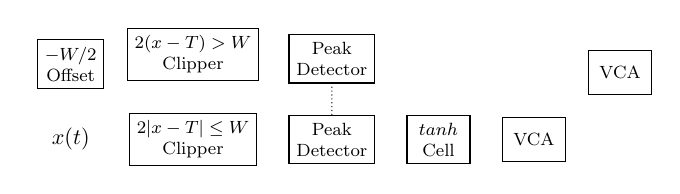
\begin{tikzpicture}[scale = 0.8, transform shape]

                            \node (input) at (0,0) {$x(t)$};
                            \node[block, right = of input] (clip+-) {$2|x-T|\leq W$\\Clipper};
                            \node[block, above = of input] (offset) {$-W/2$\\Offset};
                            \node[block, above = of clip+-] (clip-) {$2(x-T)>W$\\Clipper};
                            \node[block, right = of clip+-] (peak1) {Peak\\Detector};
                            \node[block, above = of peak1] (peak2) {Peak\\Detector};
                            \node[block, right = of peak1] (tanh) {$tanh$ \\Cell};
                            \node[block, right = of tanh] (vca1) {VCA};
                            \node[block, above right = of vca1] (vca2) {VCA};
                            

                            \draw[densely dotted] (peak1.north) -- (peak2.south);
                            
                        \end{tikzpicture}

                        \captionof{figure}{Knee control scheme}
                        \label{fig:knee-control}

                    \end{minipage}

                \subsubsection{Analog Multiplier and Dividers}
                    Leveraging the log and anti-log amplifiers explored in section \ref{sect:log-amp}, we possess the ability to execute both multiplication and division operations within the realm of analog circuitry. This unique capability stems from the fundamental principles of logarithmic computations, where the addition of two numbers in the logarithmic domain equates to their multiplication in the standard numerical domain once the anti-logarithm (exponential function) is applied to the resultant value as shown in equation \ref{eq:log-domain-add}.
                    
                        \begin{equation} \label{eq:log-domain-add}
                            10^{(\log_{10}A+\log_{10}B)}=A\times B
                        \end{equation}
                    
                    \noindent Similarly, a subtraction in the logarithmic domain corresponds to division in the conventional numerical domain as shown in equation \ref{eq:log-domain-minus}.

                        \begin{equation} \label{eq:log-domain-minus}
                            10^{(\log_{10}A-\log_{10}B)}=\frac{A}{B}
                        \end{equation}

                    \noindent Furthermore, such set of operations using log and anti-log amplifiers could be implement in the following manner.

                        \noindent
                        \begin{minipage}{\linewidth}

                            \centering

                            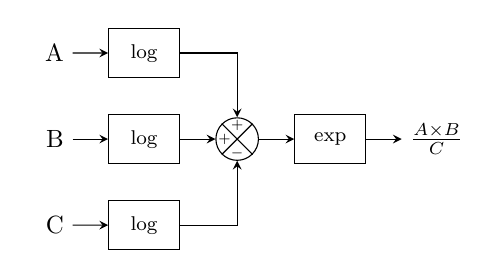
\begin{tikzpicture}[scale = 0.9, transform shape]

                                \node (input) at (0,0) {B};
                                \node[block, right = of input] (log2) {log};
                                \node[block, above = of log2] (log1) {log};
                                \node[left = of log1] (a) {A};
                                \node[block, below = of log2] (log3) {log};
                                \node[left = of log3] (c) {C};

                                % Sum1 shape
                                \node[draw,
                                    circle,
                                    minimum size=0.6cm,
                                    right = of log2,
                                ] (sum1) {};
                                \draw (sum1.north east) -- (sum1.south west) (sum1.north west) -- (sum1.south east);
                                \node[left=-1pt] at (sum1.center){\tiny $+$};
                                \node[above] at (sum1.center){\tiny $+$};
                                \node[below] at (sum1.center){\tiny $-$};

                                \node[block, right = of sum1] (exp) {exp};
                                \node[right = of exp] (out) {$\frac{A\times B}{C}$};

                                \draw[-stealth] (log1.east) -| (sum1.north);
                                \draw[-stealth] (log2.east) -- (sum1.west);
                                \draw[-stealth] (log3.east) -| (sum1.south);
                                \draw[-stealth] (sum1.east) -- (exp.west);
                                \draw[-stealth] (a.east) -- (log1.west);
                                \draw[-stealth] (input.east) -- (log2.west);
                                \draw[-stealth] (c.east) -- (log3.west);
                                \draw[-stealth] (exp.east) -- (out.west);

                            \end{tikzpicture}

                            \captionof{figure}{Multiplication and division using log and anti-log amplifiers}
                            \label{fig:pwr-mng}

                        \end{minipage}

                    \noindent Using this feature of mathematical operations, the circuit can be arranged in a way so that we can implement the output of an gain detector described in equation \ref{eq:gain-comp}.

                \subsubsection{Hyperbolic Tangent Function Cell}

                    A hyperbolic tangent function can be achieved in the analog signal domain by implementing a differential transistor pair coupled with an input of an operational amplifier.
                    As the input range of the function cell is determined by the voltage range of the active region given by the base input of the bipolar junction transistor, it is crucial to normalize the amplitude of the signal entering the cell beforehand. As seen in figure \ref{plot:tanh}, the gated nature of BJT input allows us to create unique characteristics in the definition of how the knee control is applied.

                        % tanh plot
                        \noindent
                        \begin{minipage}{\linewidth}

                            \centering
                            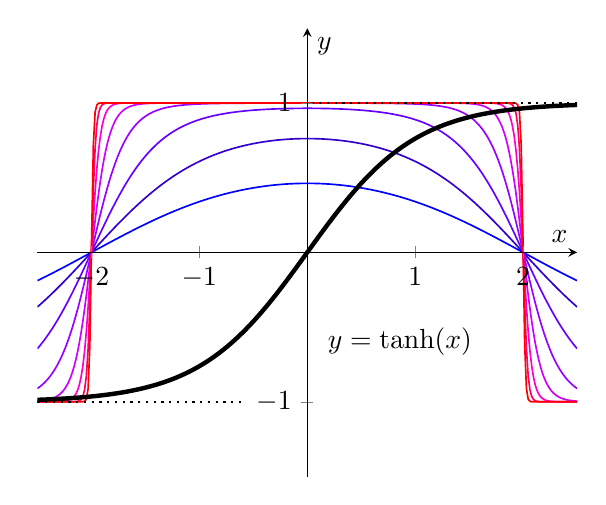
\begin{tikzpicture}
                                \begin{axis}[
                                        xmin=-2.5, xmax=2.5,
                                        ymin=-1.5, ymax=1.5,
                                        axis lines=center,
                                        axis on top=true,
                                        domain=-2.5:2.5,
                                        samples=310,
                                        ylabel=$y$,
                                        xlabel=$x$,
                                    ]
                                    \definecolor{c1}{HTML}{0000FF}
                                    \definecolor{c2}{HTML}{3300CC}
                                    \definecolor{c3}{HTML}{6600FF}
                                    \definecolor{c4}{HTML}{9900FF}
                                    \definecolor{c5}{HTML}{CC00FF}
                                    \definecolor{c6}{HTML}{FF00CC}
                                    \definecolor{c7}{HTML}{FF0066}
                                    \definecolor{c8}{HTML}{FF0000}

                                    \addplot [mark=none,draw=c1,semithick] {tanh(0.5*cos(deg(x)*1/4*pi))};
                                    \addplot [mark=none,draw=c2,semithick] {tanh(cos(deg(x)*1/4*pi))};
                                    \addplot [mark=none,draw=c3,semithick] {tanh(2*cos(deg(x)*1/4*pi))};
                                    \addplot [mark=none,draw=c4,semithick] {tanh(4*cos(deg(x)*1/4*pi))};
                                    \addplot [mark=none,draw=c5,semithick] {tanh(8*cos(deg(x)*1/4*pi))};
                                    \addplot [mark=none,draw=c6,semithick] {tanh(16*cos(deg(x)*1/4*pi))};
                                    \addplot [mark=none,draw=c7,semithick] {tanh(32*cos(deg(x)*1/4*pi))};
                                    \addplot [mark=none,draw=c8,semithick] {tanh(64*cos(deg(x)*1/4*pi))};
                                
                                    \addplot [mark=none,draw=black,ultra thick] {tanh(\x)};
                                    \node [right, black] at (axis cs:0.1,-0.6) {$y = \tanh (x)$};
                                    
                                    %% Add the asymptotes
                                    \draw [black, dotted, thick] (axis cs:-2.5,-1) -- (axis cs:-0.6,-1);
                                    \draw [black, dotted, thick] (axis cs:+2.5,+1) -- (axis cs:0,+1);
                                \end{axis}
                            \end{tikzpicture}
                                
                            \captionof{figure}{The black line shows the function plot of $y=tanh(x)$. The red line on the other hand represents the transient output of the tanh function where amplitude of the sinusoidal input is varied.}
                            \label{plot:tanh}
                        
                        \end{minipage}
            
            \subsection{Transient Shaping}

                \subsubsection{Precision Peak Detector}
                    \textcolor{blue}{This is an alternative to the RMS detector. However, it excels at fast attack signals compared to the RMS detector. This allows the compressor to process signals at higher speeds instead of simply normalizing the volume.}

                    A simple peak detection circuit can be implemented using a diode, a capacitor, and a resistor.

                \subsubsection{True RMS Detector}
                    A traditional approach to reading the average of an input signal was to implement a      
                    
                \subsubsection{Crossfader}
                    To implement the mechanism discussed in section \ref{sect:rms-peak-mix}, a crossfader can be implemented to allow an continuous 

            \subsection{Voltage Controlled Amplifier}
                A voltage controlled amplifier allows an 
                

        \section{Physical Compressor Hardware}
            This section diverges from the topics discussed in previous sections and focuses more on the technicalities involved in implementing the circuit that has been designed. Specific challenges associated with audio domain signals will be introduced to make the reader aware of anything to be cautious.
            \textcolor{blue}{I plan to use Altium Designer for designing the PCB. Describe steps taken during the PCB design process and any important points noticed.}

            \subsection{Miscellaneous Circuitry}

                \subsubsection{Power Delivery}
                    Audio domain applications gain advantages from utilizing a bipolar bias power supply. Such a supply enhances the effective utilization of IC's full dynamic range, facilitates rail-to-rail amplification, shields the analog signal from ground noise, and delivers numerous additional benefits. \cite{ti-3-v-rails}\par
                    To receive the benefits of a split rail power supply while reducing unwanted noise and ripples seen in common topologies such as a simple switching mode power supply, a topology where a inverting charge pump is combined with an linear \& low-dropout (LDO) regulator. (shown in figure)\par
                    \textcolor{blue}{Discuss the difference in LDO over traditional power regulation sources. The DRC circuit will require a DC power source that will be converted to several voltage domains (+12V, -12V, 5V).}
                    
                    % Power management scheme diagram
                    \noindent
                    \begin{minipage}{\linewidth}

                        \centering

                        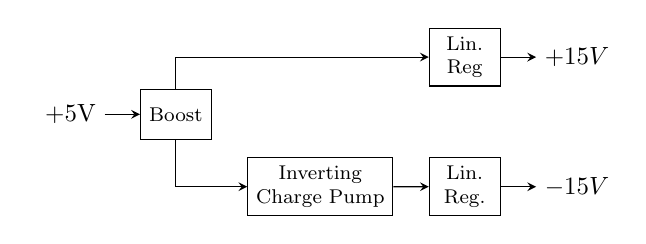
\begin{tikzpicture}[scale = 0.9, transform shape]

                            \node (input) at (0,0) {+5V};
                            \node[block, right = of input] (boost) {Boost};
                            \node[block, below right = 0.25 and 0.5 of boost] (icp) {Inverting\\Charge Pump};
                            \node[block, right = of icp] (n-ldo) {Lin.\\Reg.};
                            \node[block, above = 1 of n-ldo] (p-ldo) {Lin.\\Reg};

                            \draw[-stealth] (input) -- (boost.west);
                            \draw[-stealth] (boost.south) |- (icp.west);
                            \draw[-stealth] (boost.north) |- (p-ldo.west);
                            \draw[-stealth] (icp.east) -- (n-ldo.west);
                            \draw[-stealth] (p-ldo.east) -- +(0.5,0) node[right]{$+15V$};
                            \draw[-stealth] (n-ldo.east) -- +(0.5,0) node[right]{$-15V$};

                            %\node[block, above = of p-ldo] (p-ldo2) {Lin.\\Reg.};
                            %\draw[-stealth] (boost.north) |- (p-ldo2.west);
                            %\draw[-stealth] (p-ldo2.east) -- +(0.5,0) node[right]{$+5V$};

                        \end{tikzpicture}

                        \captionof{figure}{Power Managemenet Schema}
                        \label{fig:pwr-mng}

                    \end{minipage}

                \subsubsection{Balanced Line Input/Output}
                    The use of a balanced line driver/receiver are commonly seen in professional audio hardware, and it aids in minimizing noise and interference. The used of balanced line input and output employs differential signaling to effectively cancel out noise and electromagnetic interference picked up along cable runs, which allows  for preserving the dynamic range and subtleties of the audio signal. This setup is particularly advantageous for long cable runs and in environments with high electronic noise, ensuring that analog compressors can accurately control dynamics without the detrimental effects of added noise or signal degradation.\par
                    While differential line receivers and drivers can be designed with ease using a set of precision resistors and precision resistors, specialized ICs such as 

                \subsubsection{Precision Current Sink Source}
                    A current source is required to generate a constant ink of current across the collector and the emitter of the BJT being used in the tanh function cell.
                    We utilize the design shown in \cite{ti-sink-source}.

            \subsection{Printed Circuit Board Design}

                \subsubsection{Layer Stackup}
                    With the emergence of low-cost off-shore PCB manufacturing services, PCBs are easily in the reach of an average consumer who are looking to design and produce a small quantity of electronic hardware. Due to the low-cost of 2 layer and 4 layer PCBs, a 4 layer PCB can be selected as its flexible in the routing of traces and offer better signal integrity.\par
                    The three PCB stackups depicted in figure \ref{fig:pcb-stackup}, each offers distinct advantages for power delivery and signal integrity across dual power domains. The outer GND stackup provides superior EMI shielding by enclosing signal and power layers within ground planes, ensuring stable signal propagation but potentially increasing PDN inductance due to distant power planes. The one-sided hybrid stackup allows for a compact design, situating power close to its loads on one side but risking signal integrity due to the lack of adjacent ground planes. Finally, the inner GND stackup optimizes for both power integrity, with closely coupled power and ground planes minimizing PDN impedance, and signal integrity, as signals are tightly sandwiched between grounds, albeit at the potential cost of less effective EMI shielding compared to the outer GND configuration. Each stackup requires a tailored approach to manage the complexities of positive and negative power rails, thermal performance, and mechanical robustness.

                    % PCB stackup layer comparison
                    \begin{figure*}[ht]

                        \centering

                        \begin{subfigure}[b]{0.3333\linewidth}
                            \centering
                            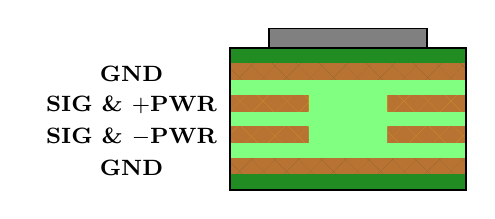
\begin{tikzpicture}
                                
                                % Light green background
                                \fill[green!50] (0,-1.4) rectangle ++(3,1);

                                % Top soldermask
                                \fill[forestgreen(web)] (0,-0.2) rectangle ++(3,0.2);

                                % S1
                                \path[fill = copper,
                                    postaction={pattern={Lines[angle=45,line width=12pt,distance={6pt}]},pattern color=forestgreen(traditional)},
                                    postaction={pattern={Lines[angle=45,line width=12pt,distance={6pt},xshift=6pt]},pattern color=copper}
                                ] (0,-0.4) rectangle ++(3,0.2);

                                % S3
                                \path[fill = red,
                                    postaction={pattern={Lines[angle=45,line width=12pt,distance={6pt}]},pattern color=yellow},
                                    postaction={pattern={Lines[angle=45,line width=12pt,distance={6pt},xshift=6pt]},pattern color=copper}
                                ] (0,-0.8) rectangle ++(1,0.2);
                                \path[fill = red,
                                    postaction={pattern={Lines[angle=45,line width=12pt,distance={6pt}]},pattern color=yellow},
                                    postaction={pattern={Lines[angle=45,line width=12pt,distance={6pt},xshift=6pt]},pattern color=copper}
                                ] (2,-0.8) rectangle ++(1,0.2);
                                
                                % S5
                                \path[fill = blue,
                                    postaction={pattern={Lines[angle=45,line width=12pt,distance={6pt}]},pattern color=yellow},
                                    postaction={pattern={Lines[angle=45,line width=12pt,distance={6pt},xshift=6pt]},pattern color=copper}
                                ] (0,-1.2) rectangle ++(1,0.2);
                                \path[fill = blue,
                                    postaction={pattern={Lines[angle=45,line width=12pt,distance={6pt}]},pattern color=yellow},
                                    postaction={pattern={Lines[angle=45,line width=12pt,distance={6pt},xshift=6pt]},pattern color=copper}
                                ] (2,-1.2) rectangle ++(1,0.2);
                                
                                % S7
                                \path[fill = copper,
                                    postaction={pattern={Lines[angle=45,line width=12pt,distance={6pt}]},pattern color=forestgreen(traditional)},
                                    postaction={pattern={Lines[angle=45,line width=12pt,distance={6pt},xshift=6pt]},pattern color=copper}
                                ] (0,-1.6) rectangle ++(3,0.2);

                                % Bottom soldermask
                                \fill[forestgreen(web)] (0,-1.8) rectangle ++(3,0.2);

                                % Outline
                                \path[draw, semithick] (0,-1.8) rectangle ++(3,1.8);

                                % Component
                                \fill[gray!100] (0.5,0) rectangle ++(2,0.25);
                                \path[draw, semithick] (0.5,0) rectangle ++(2,0.25);

                                % Labels
                                \node at (-1.25,-0.325) {\footnotesize\bf GND};
                                \node at (-1.25,-0.725) {\footnotesize\bf SIG \& $+$PWR};
                                \node at (-1.25,-1.125) {\footnotesize\bf SIG \& $-$PWR};
                                \node at (-1.25,-1.525) {\footnotesize\bf GND};

                            \end{tikzpicture}
                            \caption{{Outer GND stackup.}}
                        \end{subfigure}\hfill
                        \begin{subfigure}[b]{0.3333\linewidth}
                            \centering
                            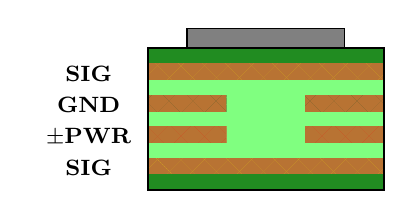
\begin{tikzpicture}
                                
                                % Light green background
                                \fill[green!50] (0,-1.4) rectangle ++(3,1);

                                % Top soldermask
                                \fill[forestgreen(web)] (0,-0.2) rectangle ++(3,0.2);

                                % S1
                                \path[fill = copper,
                                    postaction={pattern={Lines[angle=45,line width=12pt,distance={6pt}]},pattern color=yellow},
                                    postaction={pattern={Lines[angle=45,line width=12pt,distance={6pt},xshift=6pt]},pattern color=copper}
                                ] (0,-0.4) rectangle ++(3,0.2);

                                % S3
                                \path[fill = copper,
                                    postaction={pattern={Lines[angle=45,line width=12pt,distance={6pt}]},pattern color=forestgreen(traditional)},
                                    postaction={pattern={Lines[angle=45,line width=12pt,distance={6pt},xshift=6pt]},pattern color=copper}
                                ] (0,-0.8) rectangle ++(1,0.2);
                                \path[fill = copper,
                                    postaction={pattern={Lines[angle=45,line width=12pt,distance={6pt}]},pattern color=forestgreen(traditional)},
                                    postaction={pattern={Lines[angle=45,line width=12pt,distance={6pt},xshift=6pt]},pattern color=copper}
                                ] (2,-0.8) rectangle ++(1,0.2);
                                
                                % S5
                                \path[fill = blue,
                                    postaction={pattern={Lines[angle=45,line width=12pt,distance={6pt}]},pattern color=red},
                                    postaction={pattern={Lines[angle=45,line width=12pt,distance={6pt},xshift=6pt]},pattern color=copper}
                                ] (0,-1.2) rectangle ++(1,0.2);
                                \path[fill = blue,
                                    postaction={pattern={Lines[angle=45,line width=12pt,distance={6pt}]},pattern color=red},
                                    postaction={pattern={Lines[angle=45,line width=12pt,distance={6pt},xshift=6pt]},pattern color=copper}
                                ] (2,-1.2) rectangle ++(1,0.2);
                                
                                % S7
                                \path[fill = copper,
                                    postaction={pattern={Lines[angle=45,line width=12pt,distance={6pt}]},pattern color=yellow},
                                    postaction={pattern={Lines[angle=45,line width=12pt,distance={6pt},xshift=6pt]},pattern color=copper}
                                ] (0,-1.6) rectangle ++(3,0.2);

                                % Bottom soldermask
                                \fill[forestgreen(web)] (0,-1.8) rectangle ++(3,0.2);

                                % Outline
                                \path[draw, semithick] (0,-1.8) rectangle ++(3,1.8);

                                % Component
                                \fill[gray!100] (0.5,0) rectangle ++(2,0.25);
                                \path[draw, semithick] (0.5,0) rectangle ++(2,0.25);

                                % Labels
                                \node at (-0.75,-0.325) {\footnotesize\bf SIG};
                                \node at (-0.75,-0.725) {\footnotesize\bf GND};
                                \node at (-0.75,-1.125) {\footnotesize\bf $\pm$PWR};
                                \node at (-0.75,-1.525) {\footnotesize\bf SIG};

                            \end{tikzpicture}
                            \caption{{One-sided hybrid stackup.}}
                        \end{subfigure}\hfill
                        \begin{subfigure}[b]{0.3333\linewidth}
                            \centering
                            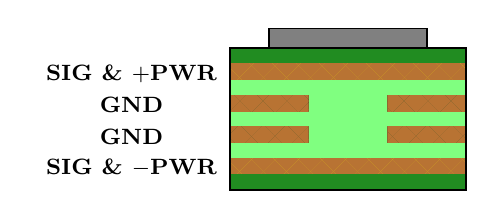
\begin{tikzpicture}
                                
                                % Light green background
                                \fill[green!50] (0,-1.4) rectangle ++(3,1);

                                % Top soldermask
                                \fill[forestgreen(web)] (0,-0.2) rectangle ++(3,0.2);

                                % S1
                                \path[fill = red,
                                    postaction={pattern={Lines[angle=45,line width=12pt,distance={6pt}]},pattern color=yellow},
                                    postaction={pattern={Lines[angle=45,line width=12pt,distance={6pt},xshift=6pt]},pattern color=copper}
                                ] (0,-0.4) rectangle ++(3,0.2);

                                % S3
                                \path[fill = copper,
                                    postaction={pattern={Lines[angle=45,line width=12pt,distance={6pt}]},pattern color=forestgreen(traditional)},
                                    postaction={pattern={Lines[angle=45,line width=12pt,distance={6pt},xshift=6pt]},pattern color=copper}
                                ] (0,-0.8) rectangle ++(1,0.2);
                                \path[fill = copper,
                                    postaction={pattern={Lines[angle=45,line width=12pt,distance={6pt}]},pattern color=forestgreen(traditional)},
                                    postaction={pattern={Lines[angle=45,line width=12pt,distance={6pt},xshift=6pt]},pattern color=copper}
                                ] (2,-0.8) rectangle ++(1,0.2);
                                
                                % S5
                                \path[fill = copper,
                                    postaction={pattern={Lines[angle=45,line width=12pt,distance={6pt}]},pattern color=forestgreen(traditional)},
                                    postaction={pattern={Lines[angle=45,line width=12pt,distance={6pt},xshift=6pt]},pattern color=copper}
                                ] (0,-1.2) rectangle ++(1,0.2);
                                \path[fill = copper,
                                    postaction={pattern={Lines[angle=45,line width=12pt,distance={6pt}]},pattern color=forestgreen(traditional)},
                                    postaction={pattern={Lines[angle=45,line width=12pt,distance={6pt},xshift=6pt]},pattern color=copper}
                                ] (2,-1.2) rectangle ++(1,0.2);
                                
                                % S7
                                \path[fill = blue,
                                    postaction={pattern={Lines[angle=45,line width=12pt,distance={6pt}]},pattern color=yellow},
                                    postaction={pattern={Lines[angle=45,line width=12pt,distance={6pt},xshift=6pt]},pattern color=copper}
                                ] (0,-1.6) rectangle ++(3,0.2);

                                % Bottom soldermask
                                \fill[forestgreen(web)] (0,-1.8) rectangle ++(3,0.2);

                                % Outline
                                \path[draw, semithick] (0,-1.8) rectangle ++(3,1.8);

                                % Component
                                \fill[gray!100] (0.5,0) rectangle ++(2,0.25);
                                \path[draw, semithick] (0.5,0) rectangle ++(2,0.25);

                                % Labels
                                \node at (-1.25,-0.325) {\footnotesize\bf SIG \& $+$PWR};
                                \node at (-1.25,-0.725) {\footnotesize\bf GND};
                                \node at (-1.25,-1.125) {\footnotesize\bf GND};
                                \node at (-1.25,-1.525) {\footnotesize\bf SIG \& $-$PWR};

                            \end{tikzpicture}
                            \caption{{Inner GND stackup.}}
                        \end{subfigure}\hfill
                        \captionof{figure}{Various PCB stackup configurations.}
                        \label{fig:pcb-stackup}
                    \end{figure*}

                \subsubsection{Component Placement}

                \subsubsection{Design Rules and Consraints}
                    The majority of design rule and constraints have been determined by referencing the tolerance specification set by the PCB manufacturer. 

                \subsubsection{Signal Integrity and EMI Precausions}

            \subsection{Component Selection}
                \textcolor{blue}{Go over components used in the circuit and why that specific part was picked. Discuss how component selection could affect thermal characteristics, linearity, bandwidth etc.}
        
        \section{Discussion}
            \textcolor{blue}{The discussion goes here.}

        \section*{Acknowledgments}
            \textcolor{blue}{Put acknowledgments here. }

        \section*{Attribution}
            \footnotesize{
                \textit{\textbf{Figure \ref{fig:comp-trans}:}} \href{https://en.wikipedia.org/wiki/Dynamic_range_compression#/media/File:Audio_Compression_Attack_and_Release-2.svg}{The attack and release phases in a compressor}, Iainf (Own work) via Wikipedia, License: \href{https://creativecommons.org/licenses/by-sa/3.0/}{CC BY-SA 3.0 DEED}\\

                \noindent\textit{\textbf{Figures \ref{fig:htan-circuit}, \ref{fig:FBR}, \ref{fig:TCPLA}, \ref{fig:peak-det-circuit}:} Schematic diagrams are generated using Altium Designer.}\\
            }

        \section*{Resources}
            All resources developed upon the completion of this project including the schematic, simulation, and CAD files are available for download at the following \textbf{\textcolor{github-butterfly-bush}{\href{https://github.com/ShaunG-RU/DRC-Project}{GitHub repository}}}, including...
            
            \begin{itemize}
                \item \href{https://github.com/ShaunG-RU/DRC-Project/blob/main/Altium/DRC.pdf}{Latest updated schematic} of the implemented analog compressor.
            \end{itemize}

        \printbibliography

        

        \iffalse
        % Diagram showing signal through the gain calculator.Takes time to compile due to increased accuracy of the plot.
        \begin{figure*}[!th]

            \centering

            \begin{minipage}[b]{0.2\linewidth}
                \centering
                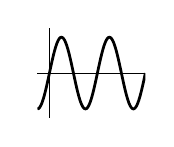
\begin{tikzpicture}[scale=0.2]
                    \begin{axis}[
                        axis lines*=middle,
                        ticks=none,
                        samples=100,
                        xmin=-0.5*pi, xmax=4*pi,
                        ymin=-1.25, ymax=1.25,
                        axis line style={line width=2pt}
                    ]
                    \addplot[
                        color=black,
                        domain=-0.5*pi:4*pi,
                        line width=5pt
                    ] {sin(deg(x))};
                    \end{axis}    
                \end{tikzpicture}
                \\
                \footnotesize{$y=sin(x)$}
            \end{minipage}\hfill

            \begin{minipage}[b]{0.2\linewidth}
                \centering
                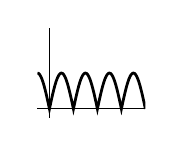
\begin{tikzpicture}[scale=0.2]
                    \begin{axis}[
                        axis lines*=middle,
                        ticks=none,
                        samples=100,
                        xmin=-0.5*pi, xmax=4*pi,
                        ymin=-0.25, ymax=2.25,
                        axis line style={line width=2pt}
                    ]
                    \addplot[
                        color=black,
                        domain=-0.5*pi:4*pi,
                        line width=5pt
                    ] {abs(sin(deg(x)))};
                    \end{axis}    
                \end{tikzpicture}
                \\
                \footnotesize{$y=\left\lvert x \right\rvert$}
            \end{minipage}\hfill

            \begin{minipage}[b]{0.2\linewidth}
                \centering
                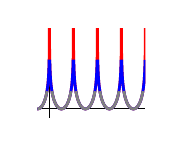
\begin{tikzpicture}[scale=0.2]
                    \begin{axis}[
                        axis lines*=middle,
                        ticks=none,
                        samples=1000,
                        xmin=-0.5*pi, xmax=4*pi,
                        ymin=-0.25, ymax=2.25,
                        axis line style={line width=2pt}
                    ]
                    \addplot[
                        color=red,
                        domain=-0.5*pi:4*pi,
                        line width=5pt
                    ] {-log10(abs(sin(deg(x))))};
                    \addplot[
                        color=blue,
                        domain=-0.5*pi:4*pi,
                        restrict y to domain=0:1.5,
                        line width=5pt
                    ] {-log10(abs(sin(deg(x))))};
                    \addplot[
                        color=black!50,
                        domain=-0.5*pi:4*pi,
                        restrict y to domain=0:0.5,
                        line width=5pt
                    ] {-log10(abs(sin(deg(x))))};
                    \end{axis}    
                \end{tikzpicture}
                \\
                \footnotesize{$y=-\log _{10}(x)$}
            \end{minipage}\hfill

            \begin{minipage}[b]{0.2\linewidth}
                \centering
                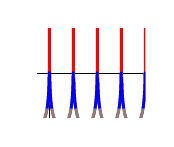
\begin{tikzpicture}[scale=0.2]
                    \begin{axis}[
                        axis lines*=middle,
                        ticks=none,
                        samples=1000,
                        xmin=-0.5*pi, xmax=4*pi,
                        ymin=-1.25, ymax=1.25,
                        axis line style={line width=2pt}
                    ]
                    \addplot[
                        color=red,
                        domain=-0.5*pi:4*pi,
                        line width=5pt
                    ] {-log10(abs(sin(deg(x))))-1.5};
                    \addplot[
                        color=black!50,
                        domain=-0.5*pi:4*pi,
                        restrict y to domain=-2:0.05,
                        line width=5pt
                    ] {-log10(abs(sin(deg(x))))-1.5};
                    \addplot[
                        color=blue,
                        domain=-0.5*pi:4*pi,
                        restrict y to domain=-1:0.05,
                        line width=5pt
                    ] {-log10(abs(sin(deg(x))))-1.5};
                    \end{axis}    
                \end{tikzpicture}
                \\
                \footnotesize{$y=x-T-\frac{W}{2}$}
            \end{minipage}\hfill

            \begin{minipage}[b]{0.2\linewidth}
                \centering
                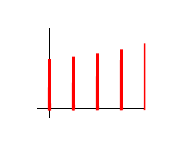
\begin{tikzpicture}[scale=0.2]
                    \begin{axis}[
                        axis lines*=middle,
                        ticks=none,
                        samples=5000,
                        xmin=-0.5*pi, xmax=4*pi,
                        ymin=-0.25, ymax=2.25,
                        axis line style={line width=2pt}
                    ]
                    \addplot[
                        color=red,
                        domain=-0.5*pi:4*pi,
                        line width=5pt,
                        restrict y to domain=-0.05:2.25,
                    ] {-log10(abs(sin(deg(x))))-1.5};
                    \end{axis}    
                \end{tikzpicture}
                \\
                \footnotesize{$y=\geq 0$}
            \end{minipage}\hfill

            \begin{minipage}[b]{0.2\linewidth}
                \centering
                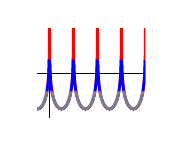
\begin{tikzpicture}[scale=0.2]
                    \begin{axis}[
                        axis lines*=middle,
                        ticks=none,
                        samples=1000,
                        xmin=-0.5*pi, xmax=4*pi,
                        ymin=-1.25, ymax=1.25,
                        axis line style={line width=2pt}
                    ]
                    \addplot[
                        color=red,
                        domain=-0.5*pi:4*pi,
                        line width=5pt
                    ] {-log10(abs(sin(deg(x))))-1};
                    \addplot[
                        color=blue,
                        domain=-0.5*pi:4*pi,
                        restrict y to domain=-1:0.5,
                        line width=5pt
                    ] {-log10(abs(sin(deg(x))))-1};
                    \addplot[
                        color=black!50,
                        domain=-0.5*pi:4*pi,
                        restrict y to domain=-1:-0.5,
                        line width=5pt
                    ] {-log10(abs(sin(deg(x))))-1};
                    \end{axis}    
                \end{tikzpicture}
                \\
                \footnotesize{$y=x-T$}
            \end{minipage}\hfill

            \begin{minipage}[b]{0.2\linewidth}
                \centering
                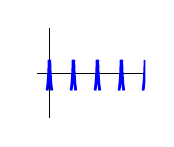
\begin{tikzpicture}[scale=0.2]
                    \begin{axis}[
                        axis lines*=middle,
                        ticks=none,
                        samples=1000,
                        xmin=-0.5*pi, xmax=4*pi,
                        ymin=-1.25, ymax=1.25,
                        axis line style={line width=2pt}
                    ]
                    \addplot[
                        color=blue,
                        domain=-0.5*pi:4*pi,
                        restrict y to domain=-0.5:0.5,
                        line width=5pt
                    ] {-log10(abs(sin(deg(x))))-1};
                    \end{axis}    
                \end{tikzpicture}
                \\
                \footnotesize{$-\frac{W}{2}\leq y \leq\frac{W}{2}$}
            \end{minipage}\hfill

            \begin{minipage}[b]{0.2\linewidth}
                \centering
                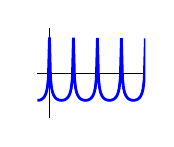
\begin{tikzpicture}[scale=0.2]
                    \begin{axis}[
                        axis lines*=middle,
                        ticks=none,
                        samples=100,
                        xmin=-0.5*pi, xmax=4*pi,
                        ymin=-1.25, ymax=1.25,
                        axis line style={line width=2pt}
                    ]
                    \addplot[
                        color=blue,
                        domain=-0.5*pi:4*pi,
                        line width=5pt
                    ] {tanh(-log10(abs(sin(deg(x))))-1)};
                    \end{axis}    
                \end{tikzpicture}
                \\
                \footnotesize{$y=tanh(x)$}
            \end{minipage}\hfill

            \caption{Transient signal throughout the attenuation calculator.}
            \label{fig:drc-diagram}

        \end{figure*}
        \fi

    \end{multicols*}

    \newpage

    \section*{Addendum}

        % Hyperbolic tangent function cell
        \noindent
        \begin{figure}[h]
            \centering
            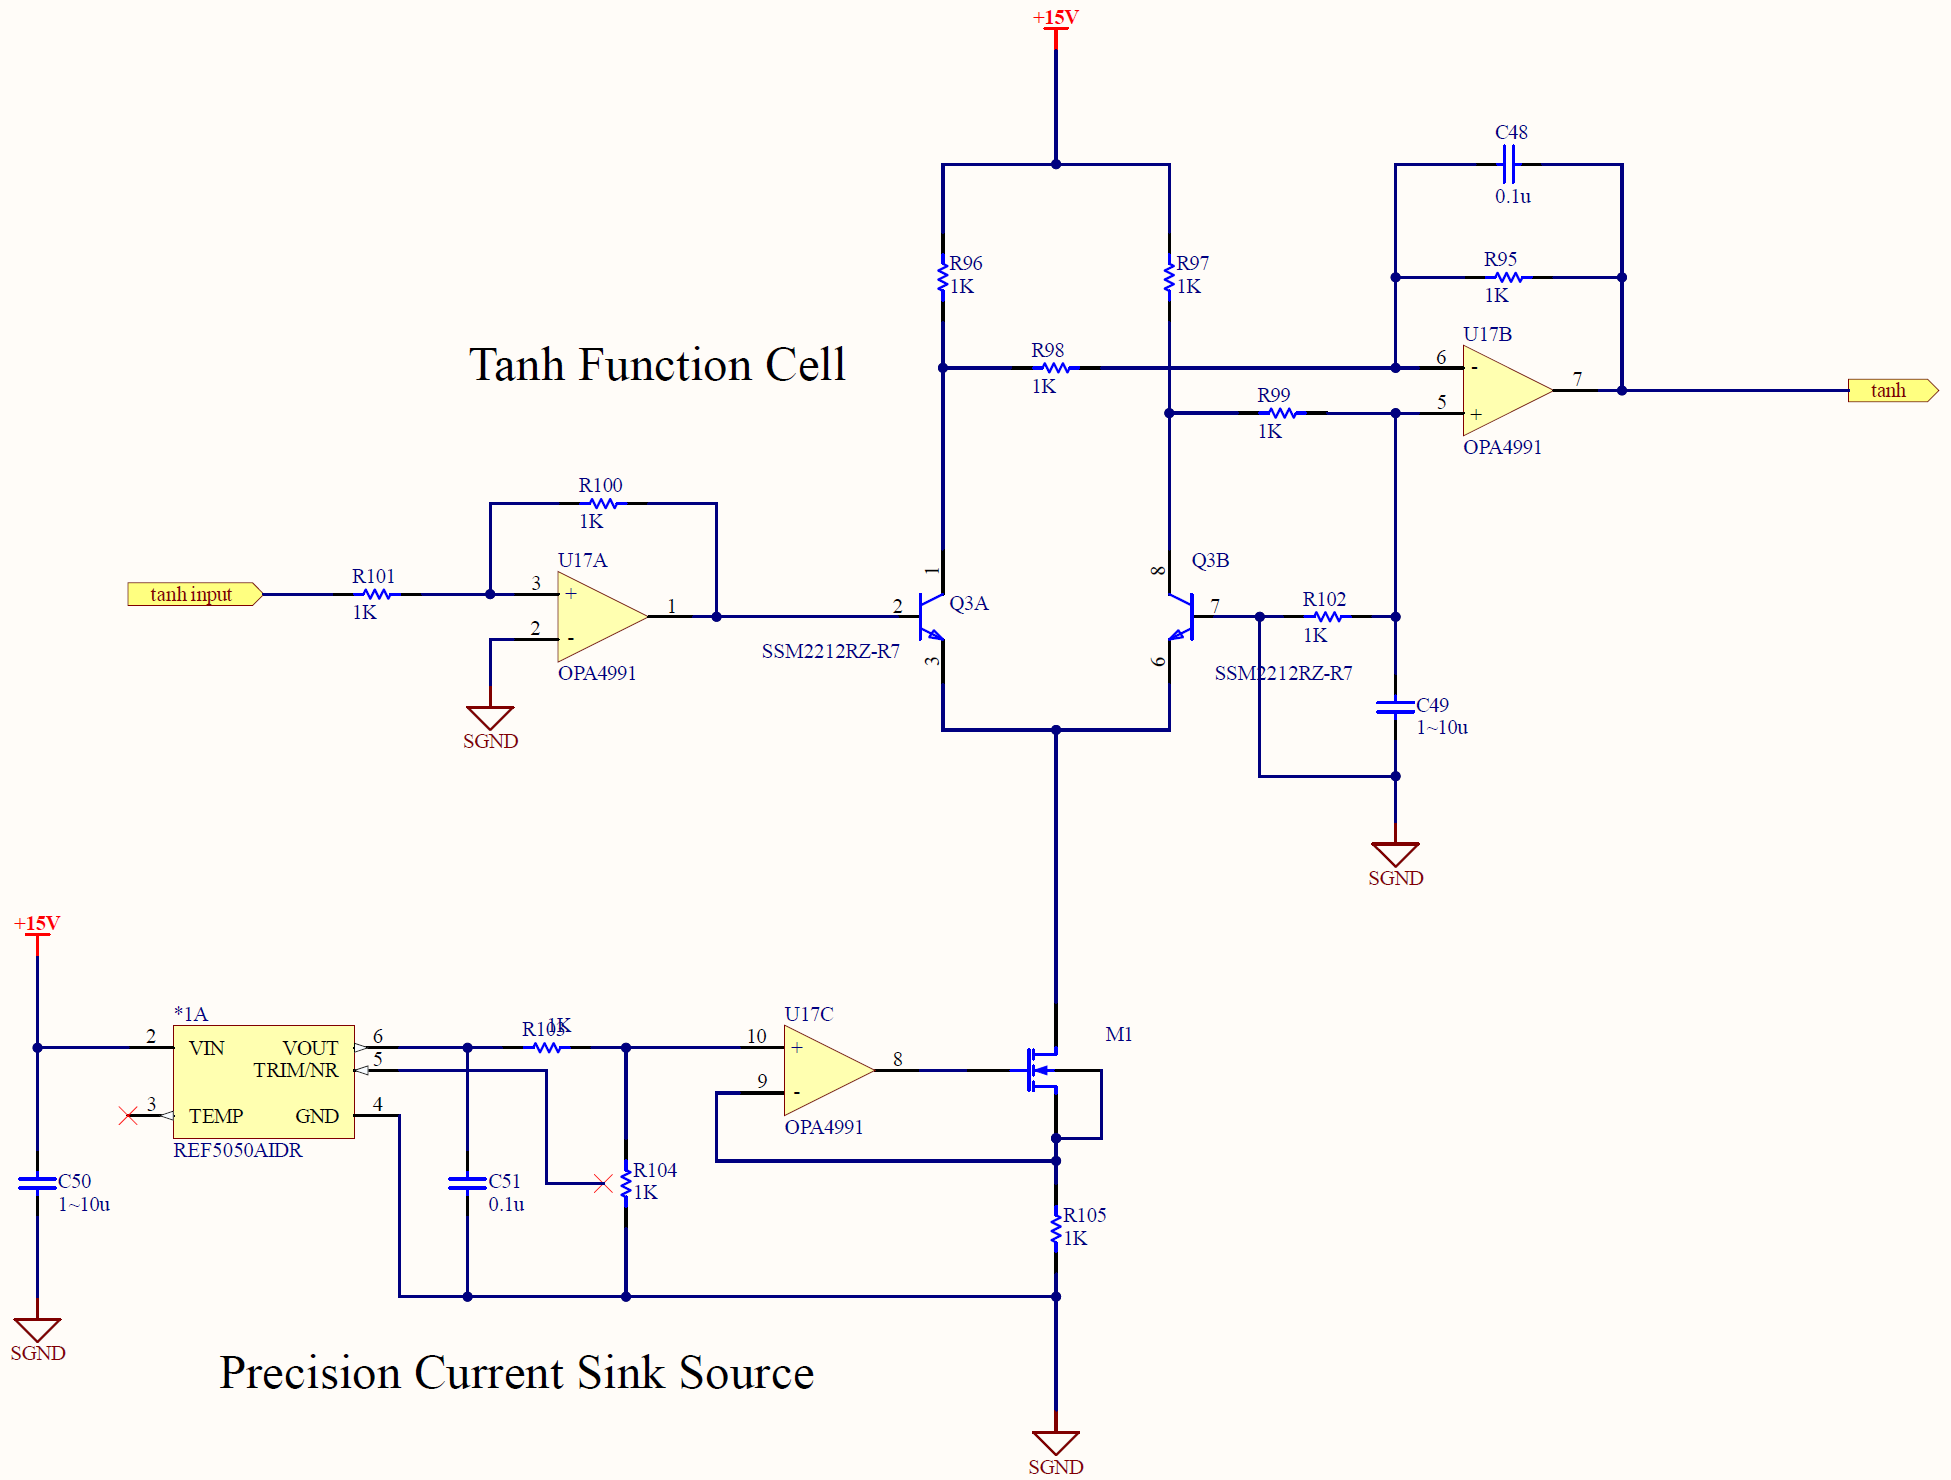
\includegraphics[width=\textwidth]{htan-circuit.png}
            \captionof{figure}{Circuit implementation of the hyperbolic tangent function cell.}
            \label{fig:htan-circuit}
        \end{figure}
        
        \vspace{-5ex}

        % Full bridge rectifier
        \noindent
        \begin{figure}[h]
            \centering
            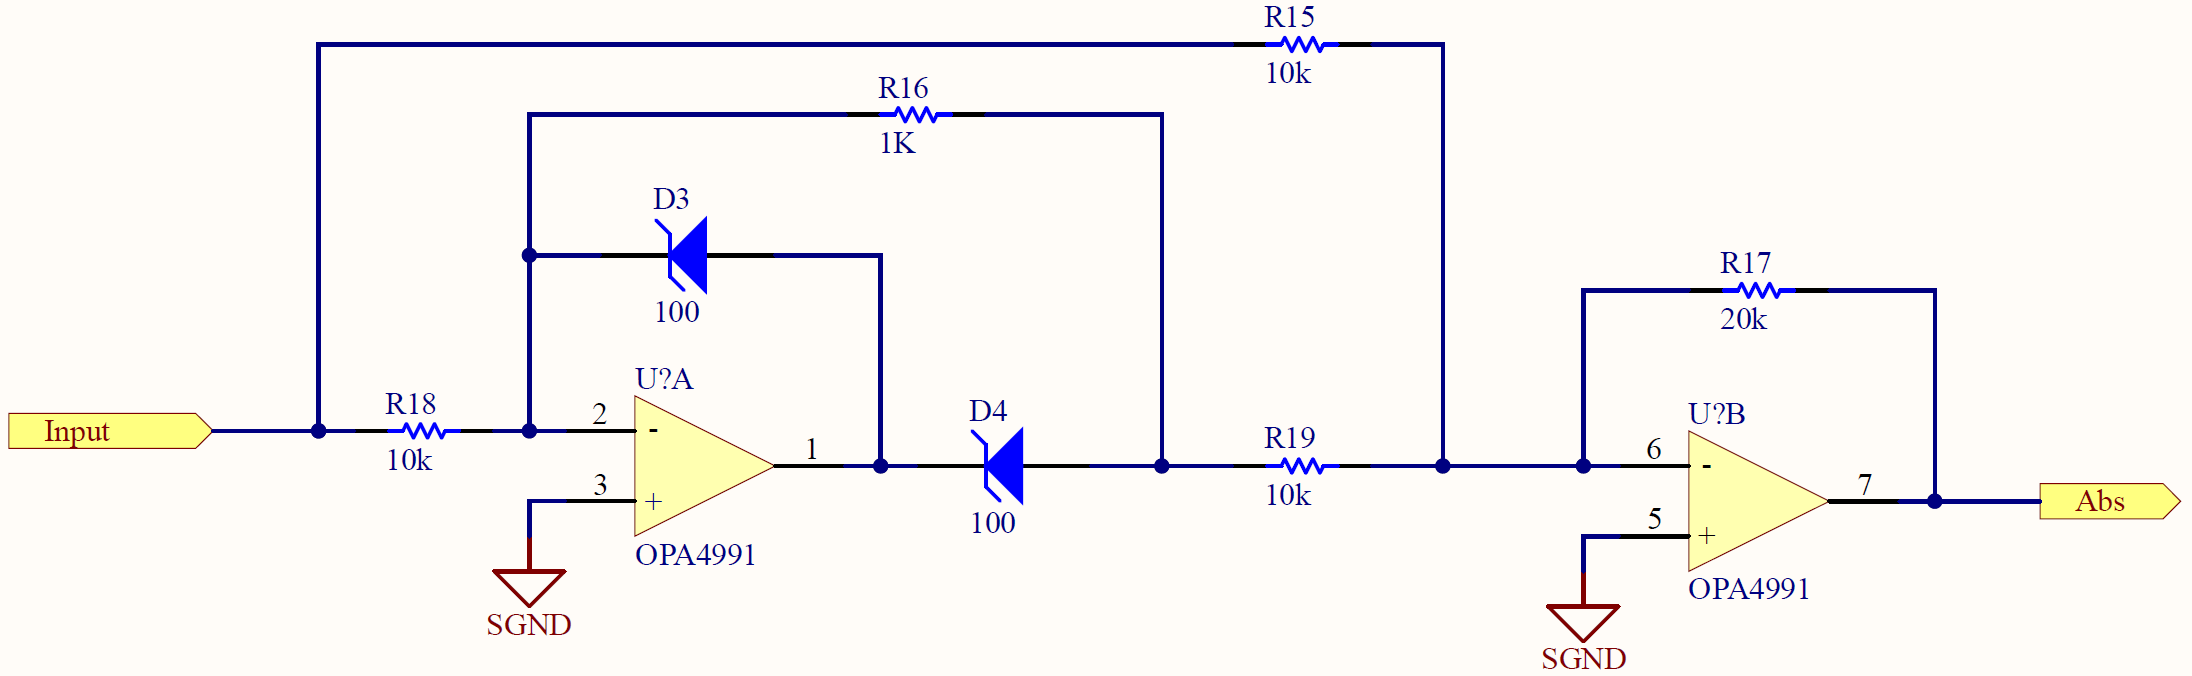
\includegraphics[width=\textwidth]{FBR-circuit.png}
            \captionof{figure}{Circuit diagram of a precision full bridge rectifier implemented in the design.}
            \label{fig:FBR}
        \end{figure}

        \vspace{-5ex}

        % Temperature compensated precision log amplifier
        \noindent
        \begin{figure}[h]
            \centering
            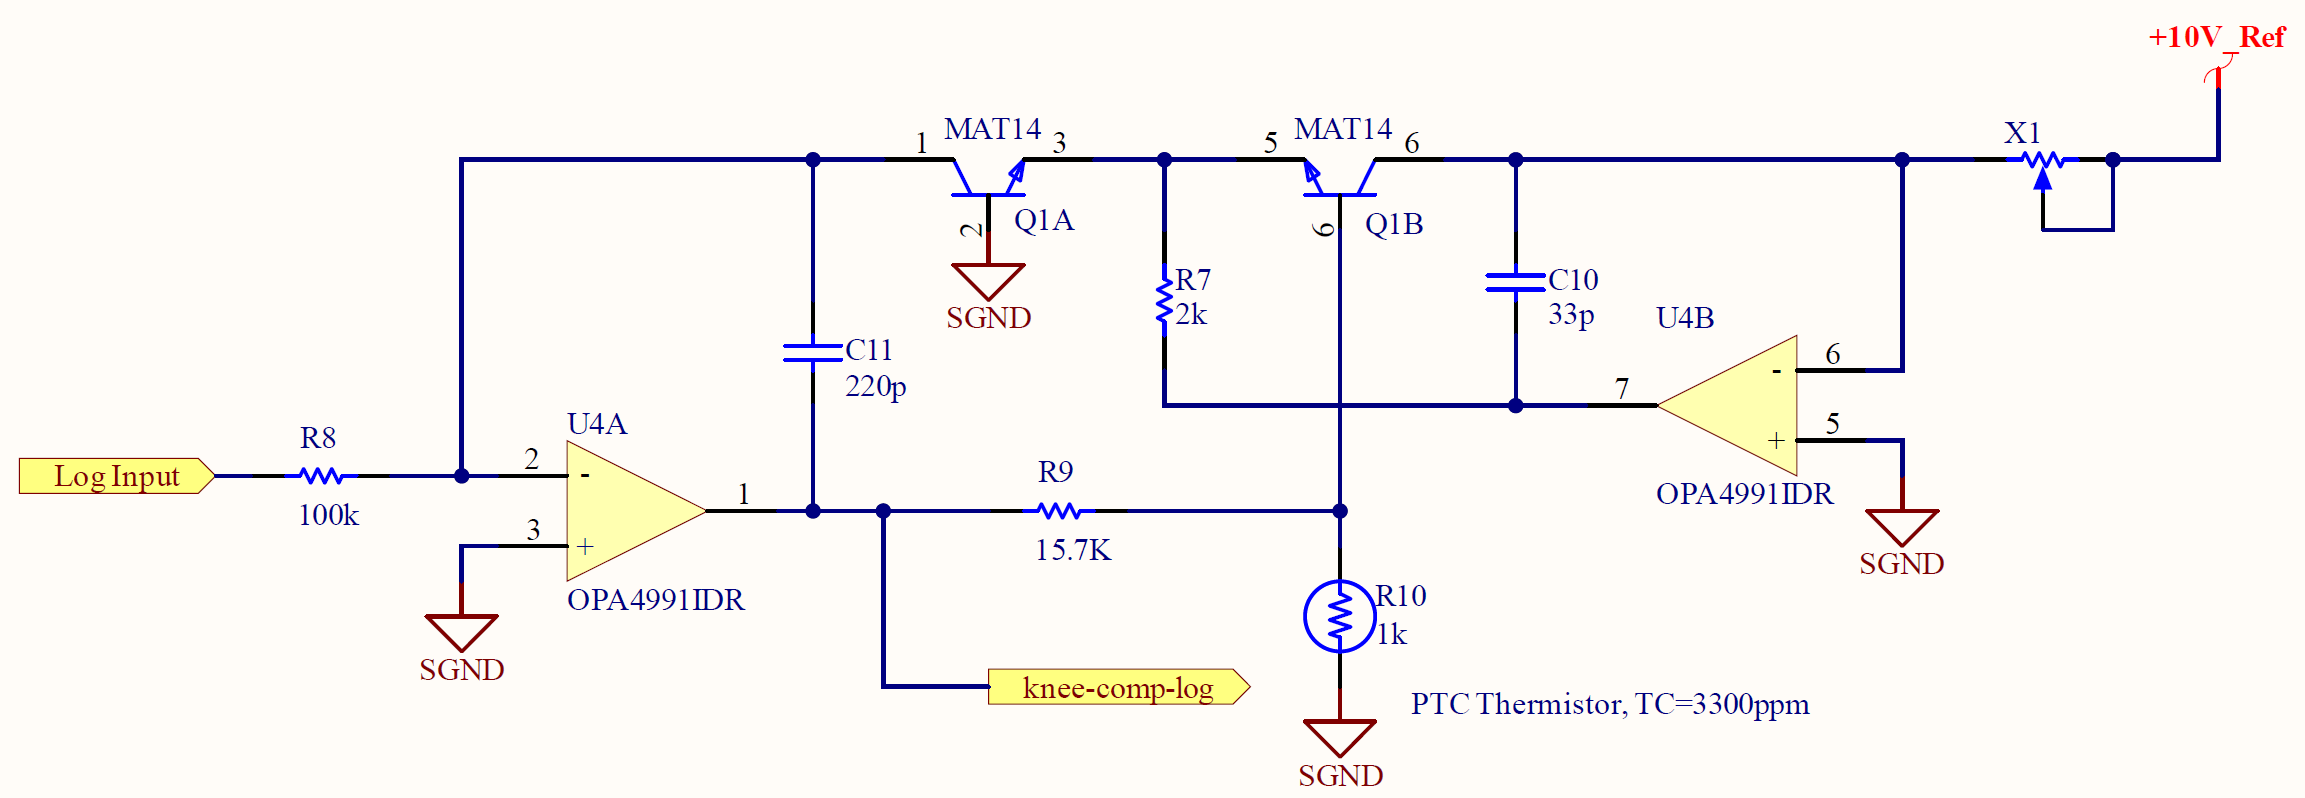
\includegraphics[width=\textwidth]{temp-comp-log-amp.png}
            \captionof{figure}{Circuit diagram of a temperature compensated precision log amplifier.}
            \label{fig:TCPLA}
        \end{figure}

        \vspace{-5ex}

        % 
        \noindent
        \begin{figure}[h]
            \centering
            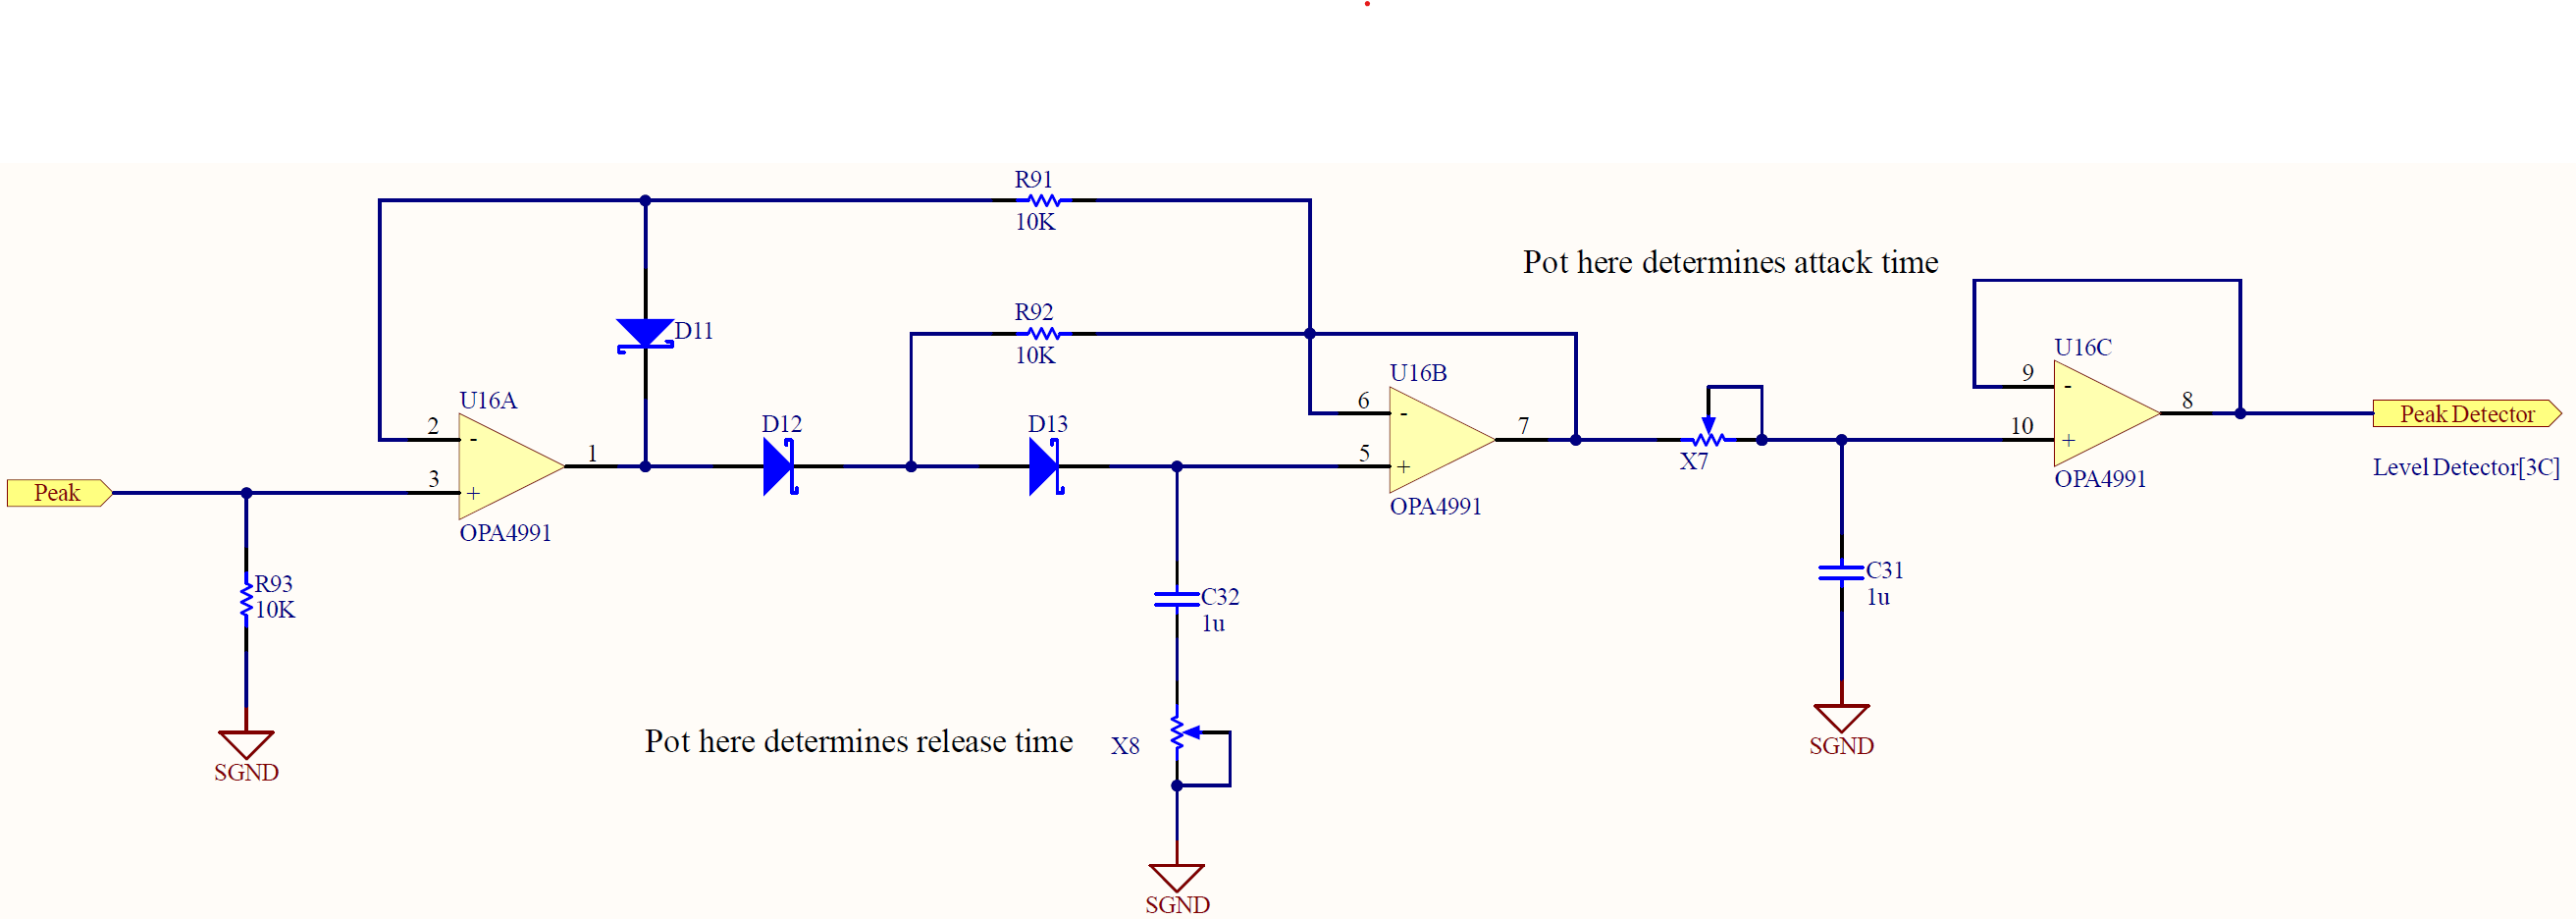
\includegraphics[width=\textwidth]{peak-detector.png}
            \captionof{figure}{Circuit diagram of an peak detector circuit with adjustable attack and release}
            \label{fig:peak-det-circuit}
        \end{figure}

        

\end{document}